\chapter{Technical}
\label{tech}

\section{ What is the average size of a move: Small, medium, large.}
We consider hourly data over the from the past 3 years.
We define 
\begin{itemize}
\item A small move to be that the range is between 1 and 2 std.
\item A medium move to be that the range is between 2 and 3 std.
\item A big move to be that the range is between $>3$ std.
\end{itemize}
\begin{verbatim}
1 std 8.159378637671352
2 std 16.318757275342705
3 std 24.478135913014057
\end{verbatim}

Figure \ref{fig:move} plot the range distribution along with its stds.

\begin{figure}[H]
\center
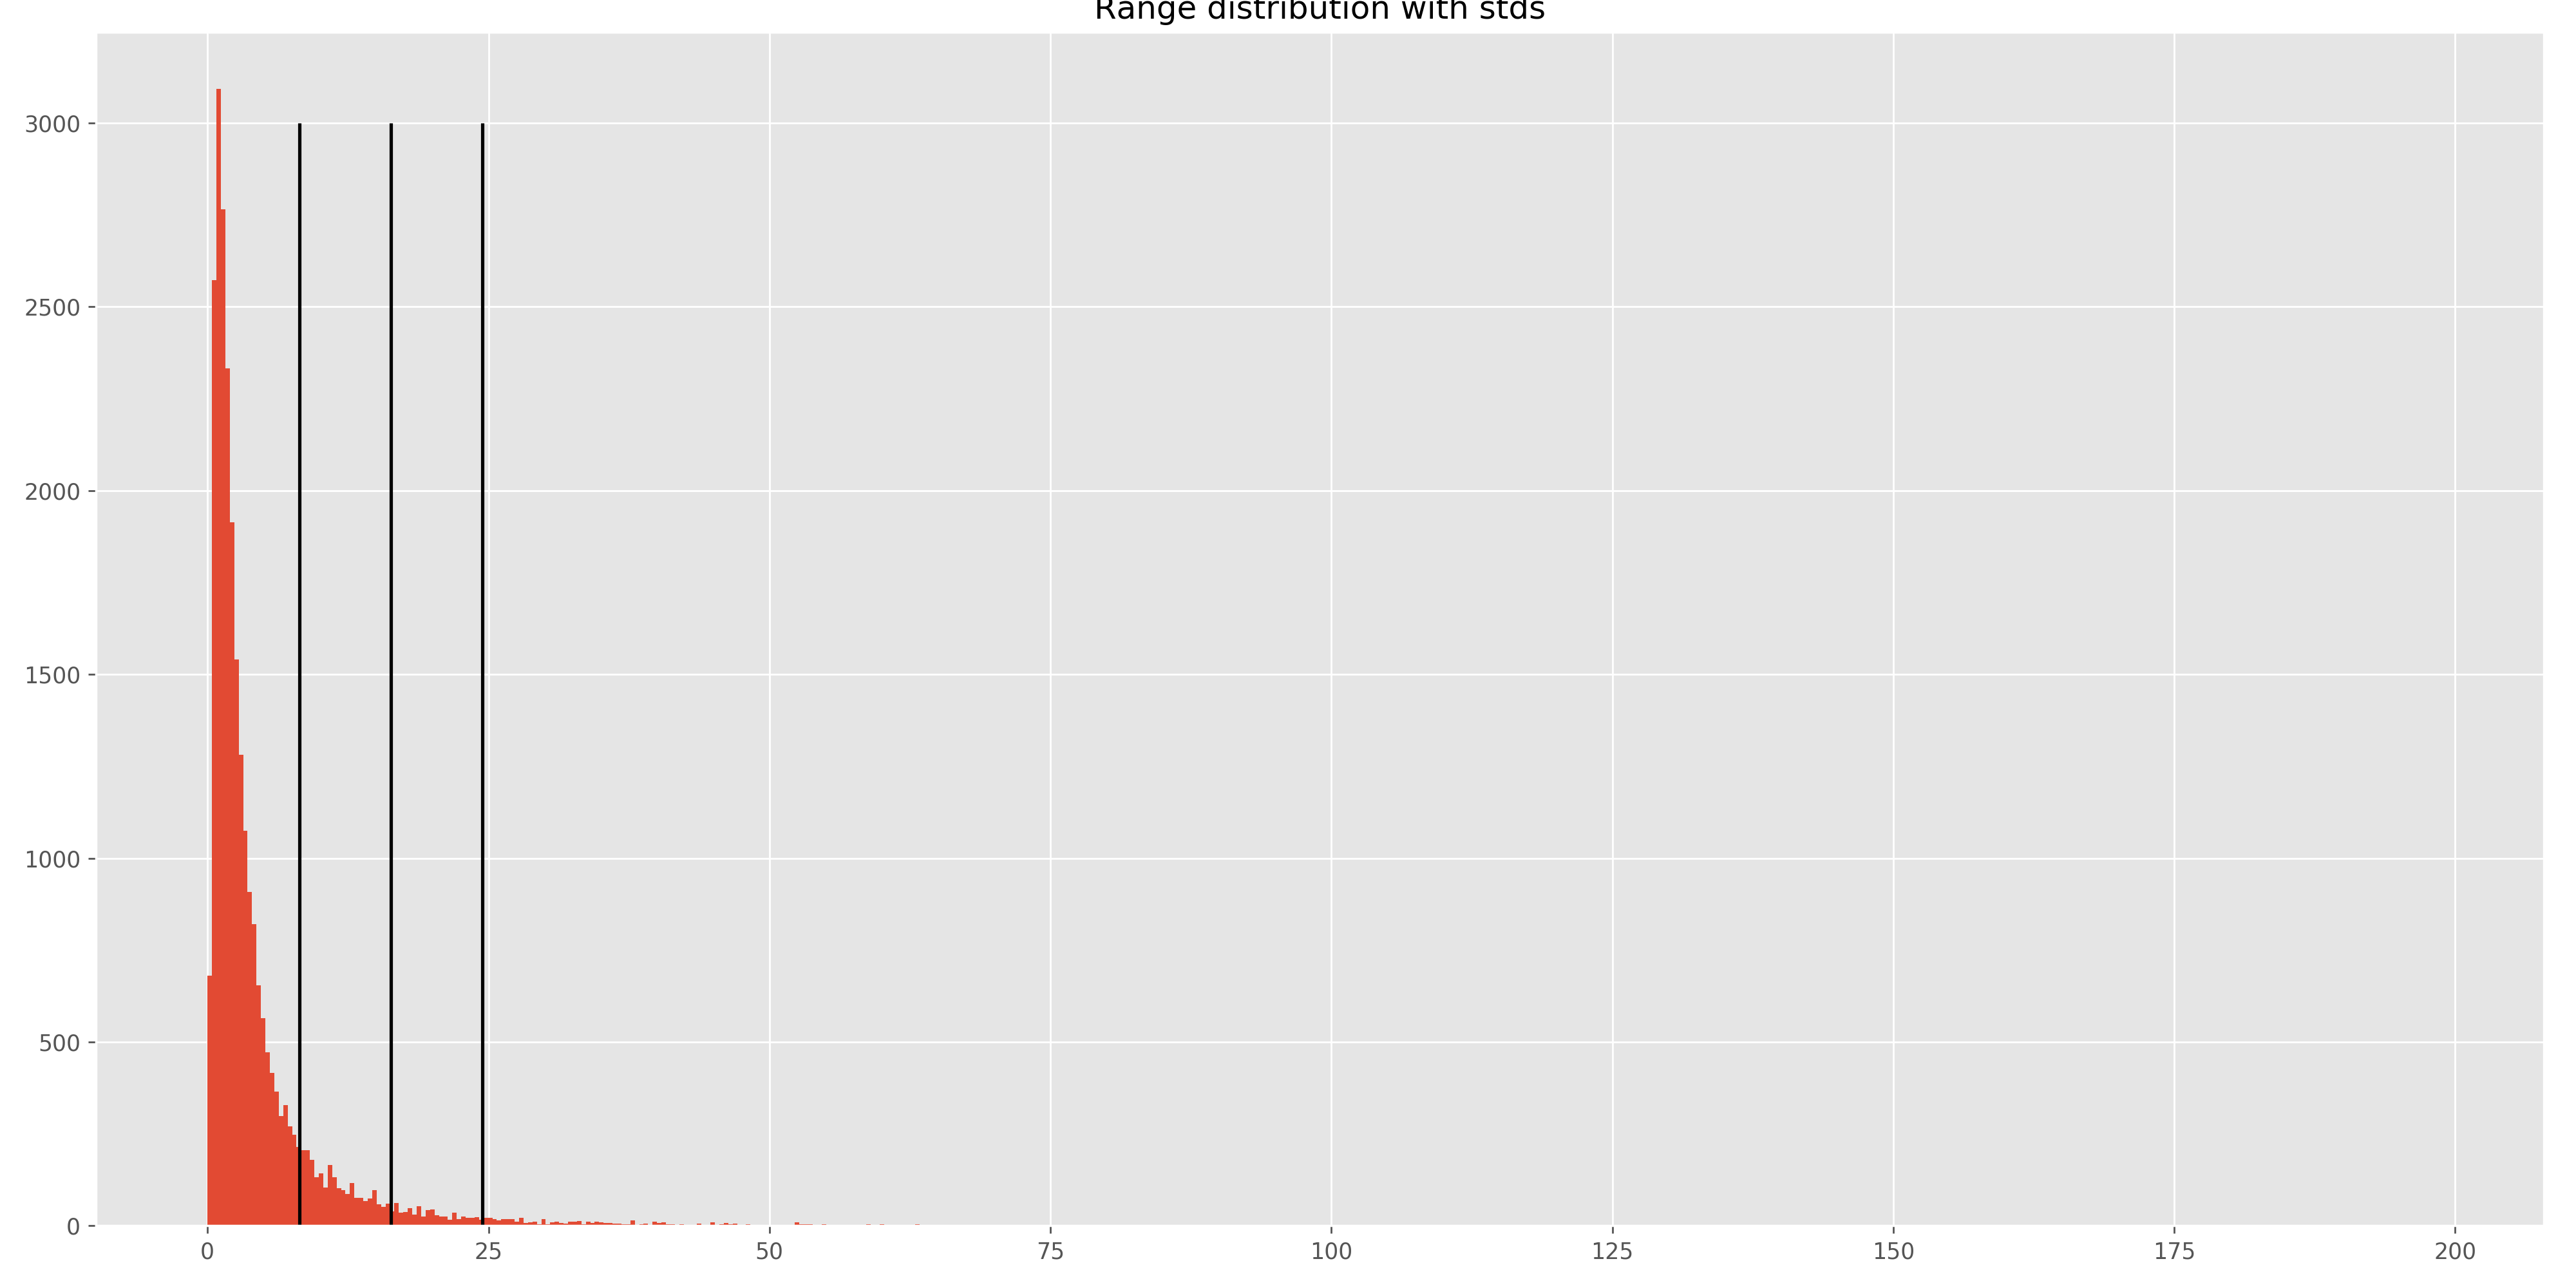
\includegraphics[width=0.9\textwidth]{fig/move.png}
\caption{Range distribution over the last 3 years for hourly data along with its stds}
\label{fig:move}
\end{figure}
\section{ Most amount of candles in a row with one color}
We consider hourly data over the from the past 3 years.

We define
\begin{itemize}
\item A green candle  :  $close(t) > open(t)$
\item A red candle  :  $close(t) < open(t)$
\end{itemize}
The most in a row with one color is green. This happen on '2017-10-06 12:00:00' to '2017-10-06 23:00:00' (inclusive) for 12 candles

Here is the algorithm used to count candles

\begin{verbatim}
def candle_in_row(is_green):
    """
    takes a pandas series returns a np.array
    """
    
    count = 1
    in_row = np.ones(len(is_green))
    for i in range(1,len(is_green)):
        if is_green[i] == is_green[i-1]:
            count += 1
            in_row[i] = count
        else:
            count = 1
            in_row[i] = count
    return in_row 
\end{verbatim}
\section{ Does the market respond to triangles / wedges?}
This questions is answered qualitatively (find patterns by hand)

We find that there more triangles / wedges followed by a break out on all time frames.

Here are some examples
\begin{figure}[H]
\center
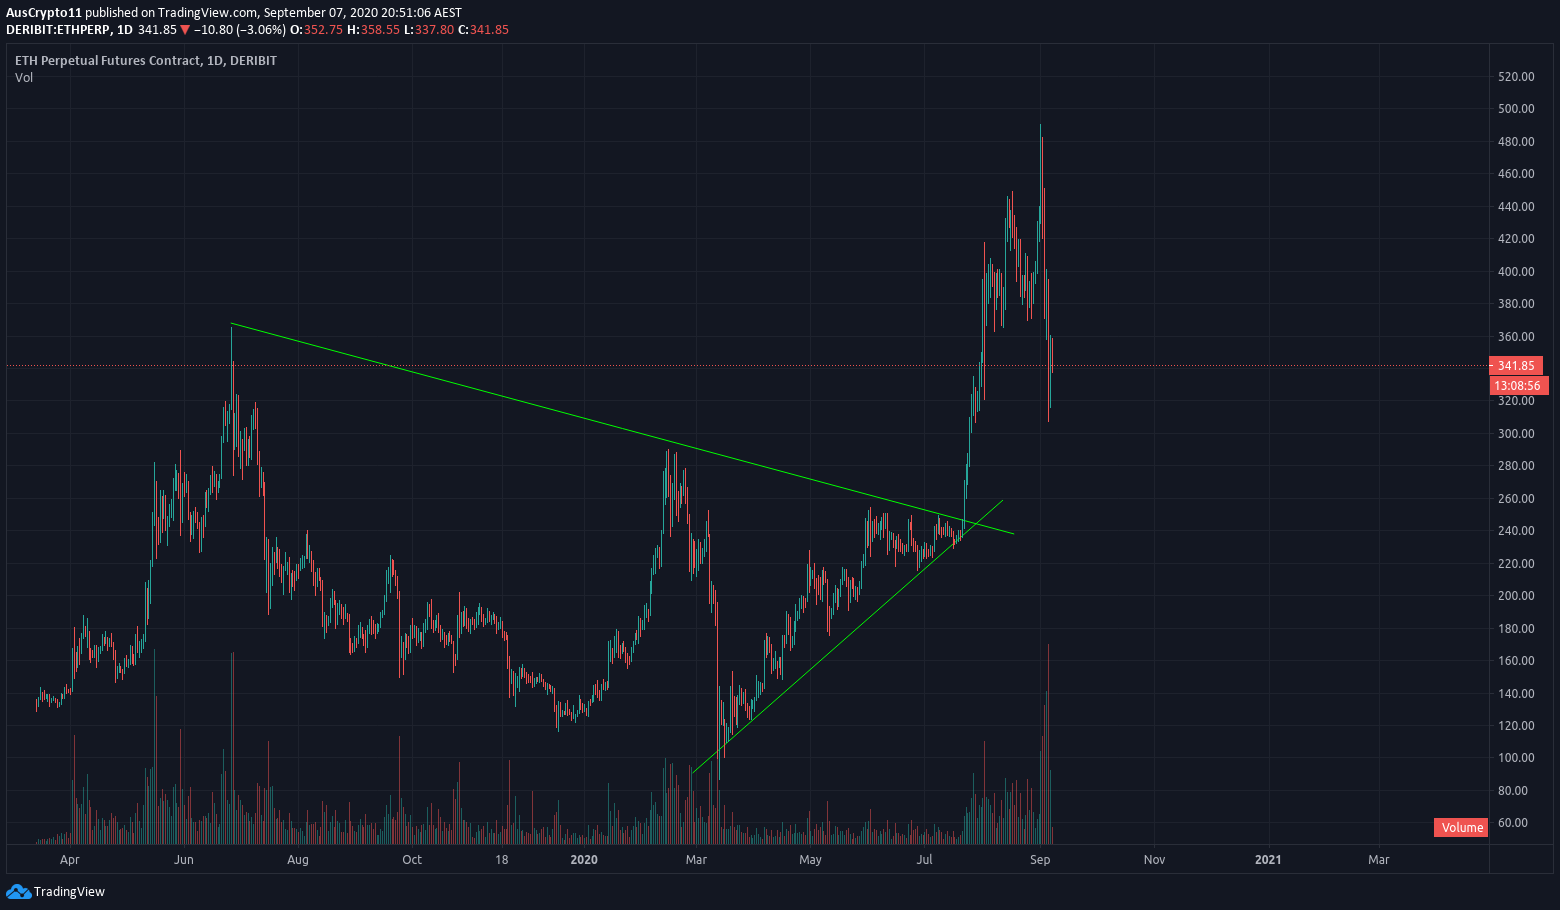
\includegraphics[width=0.8\textwidth]{fig/tri/t1.png}
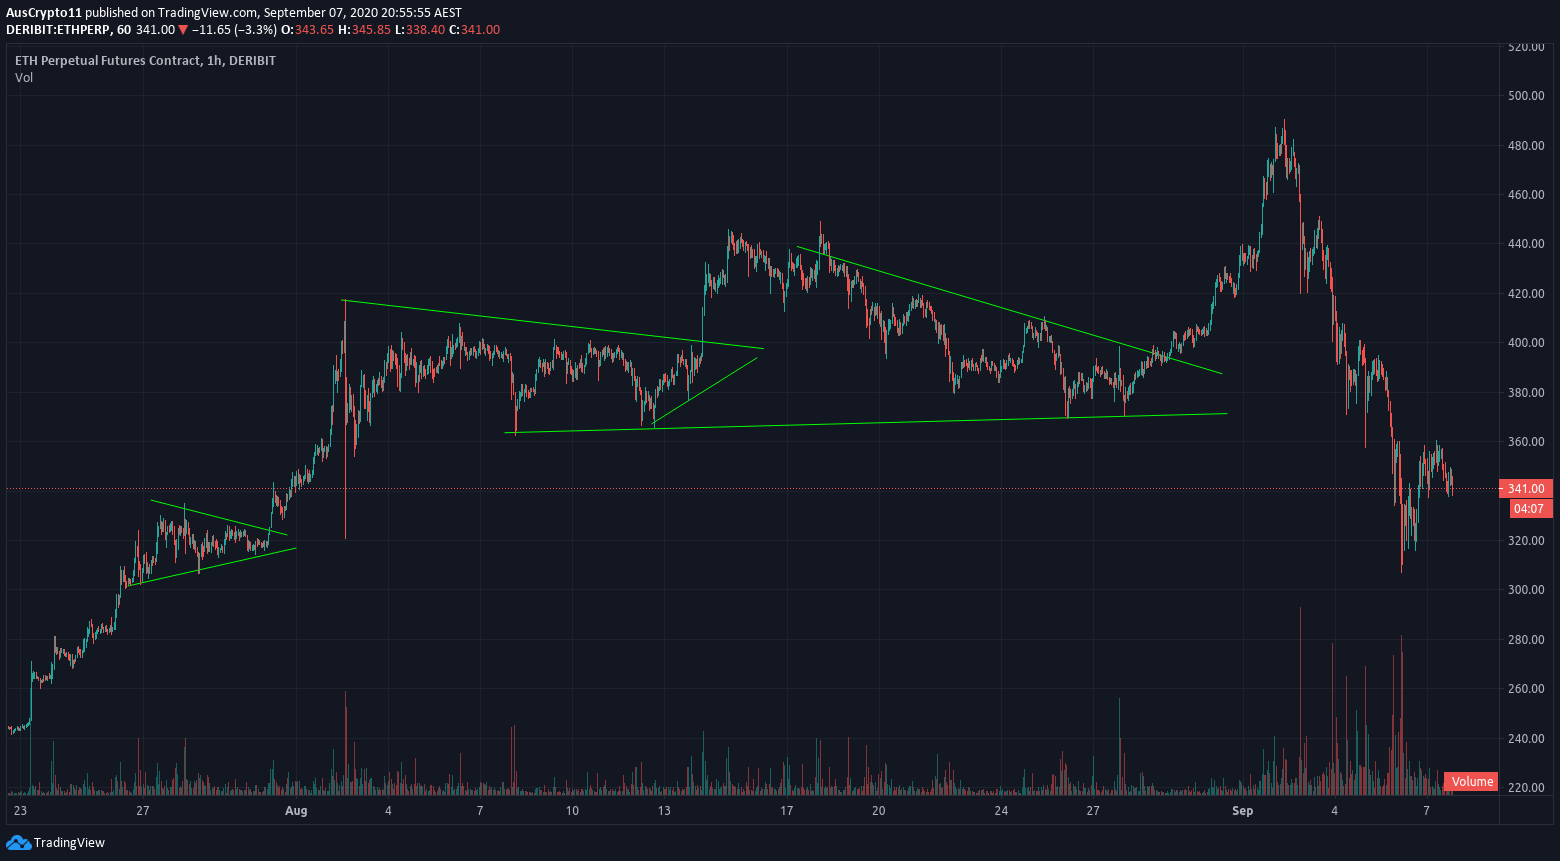
\includegraphics[width=0.8\textwidth]{fig/tri/t2.png}
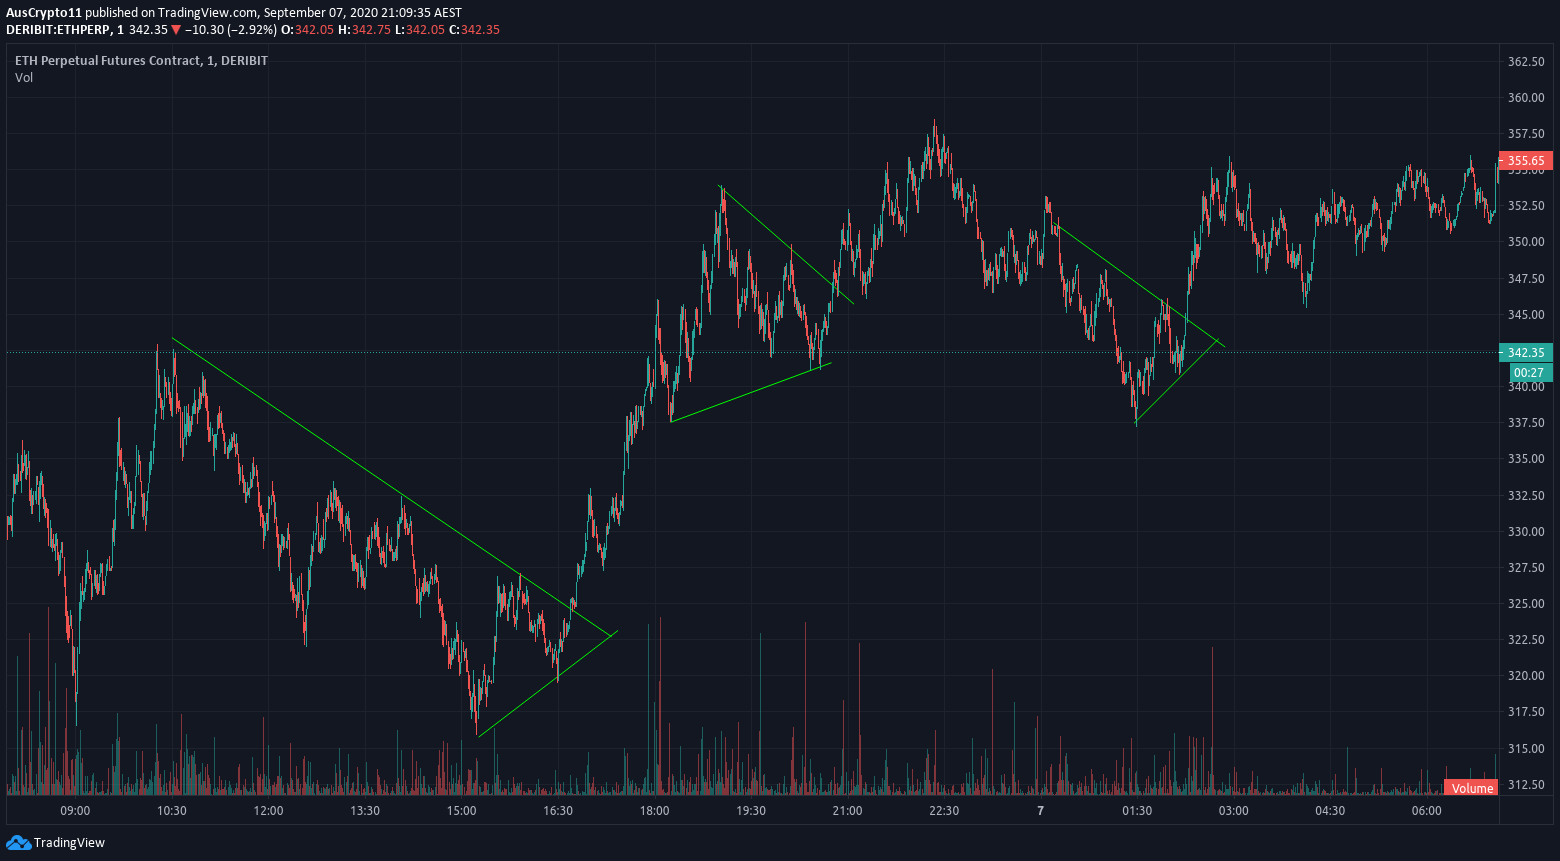
\includegraphics[width=0.8\textwidth]{fig/tri/t3.png}
\caption{triangles / wedges}

\end{figure}

\begin{figure}[H]
\center
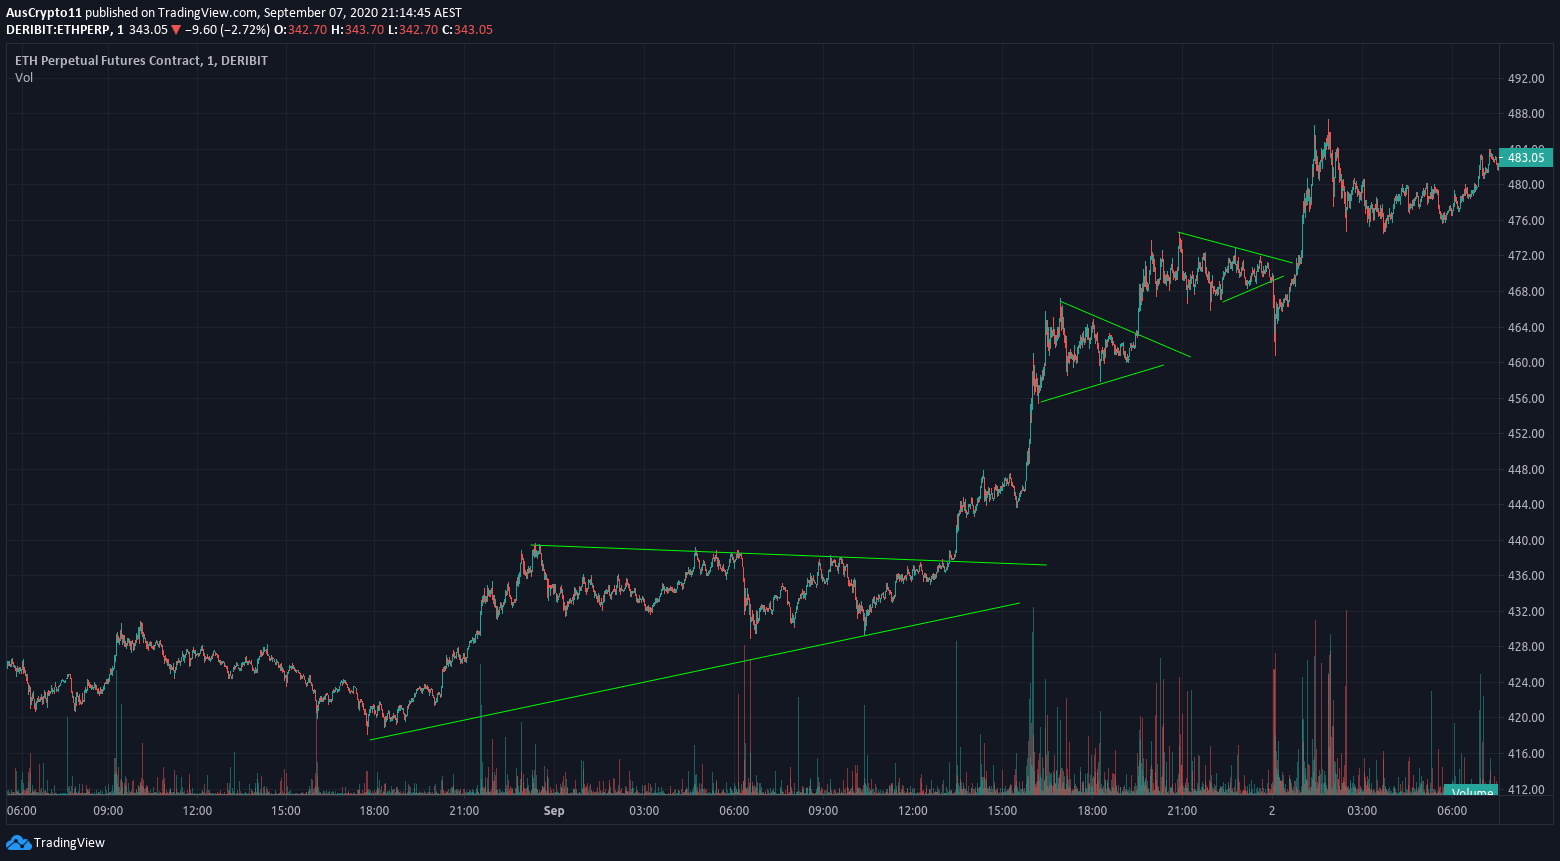
\includegraphics[width=0.8\textwidth]{fig/tri/t4.png}
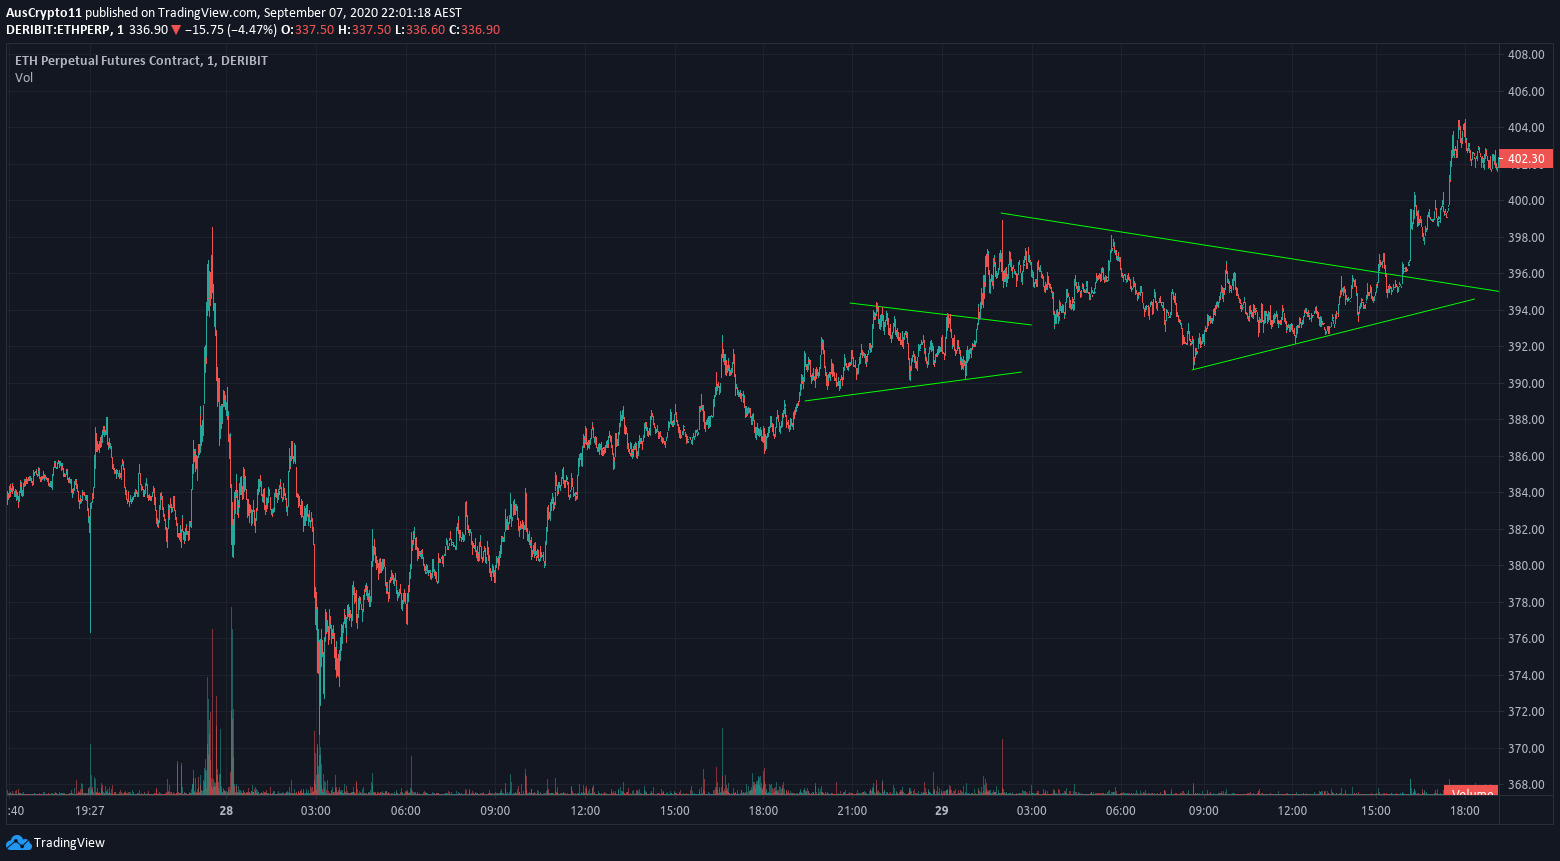
\includegraphics[width=0.8\textwidth]{fig/tri/t5.png}
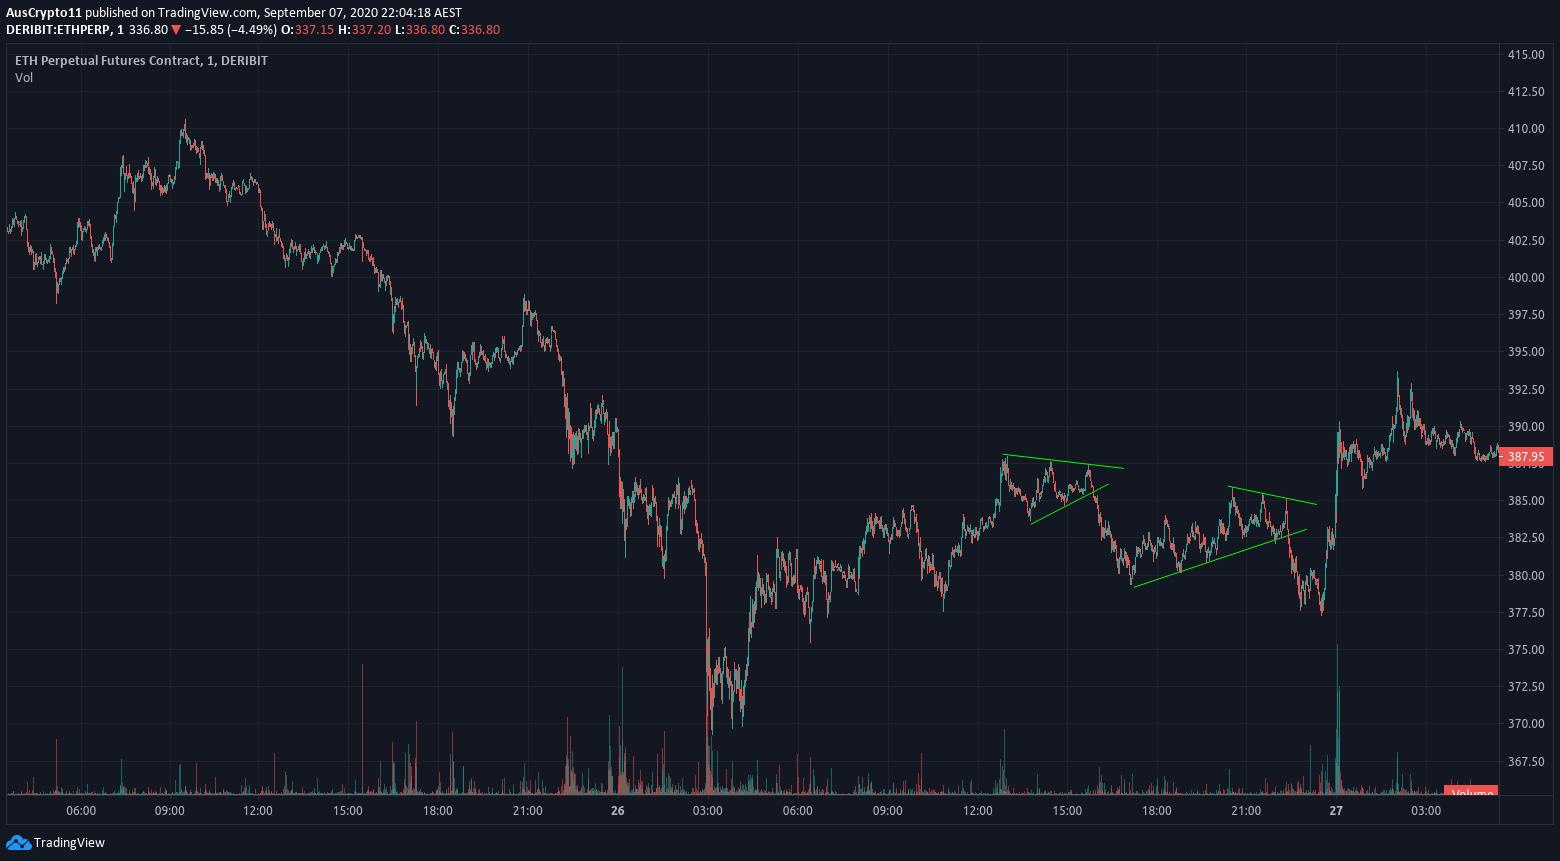
\includegraphics[width=0.8\textwidth]{fig/tri/t6.png}
\caption{triangles / wedges}
\end{figure}
\section{ Does the market respond to flags? bull flags vs bear flags, flat flags. }

This questions is answered qualitatively (find patterns by hand)

Flag seem to only appear on the shorter time frames. In the last week the have been very few.
However there seem to be more bull flags than bear flags
Here are some examples

\begin{figure}[H]
\center
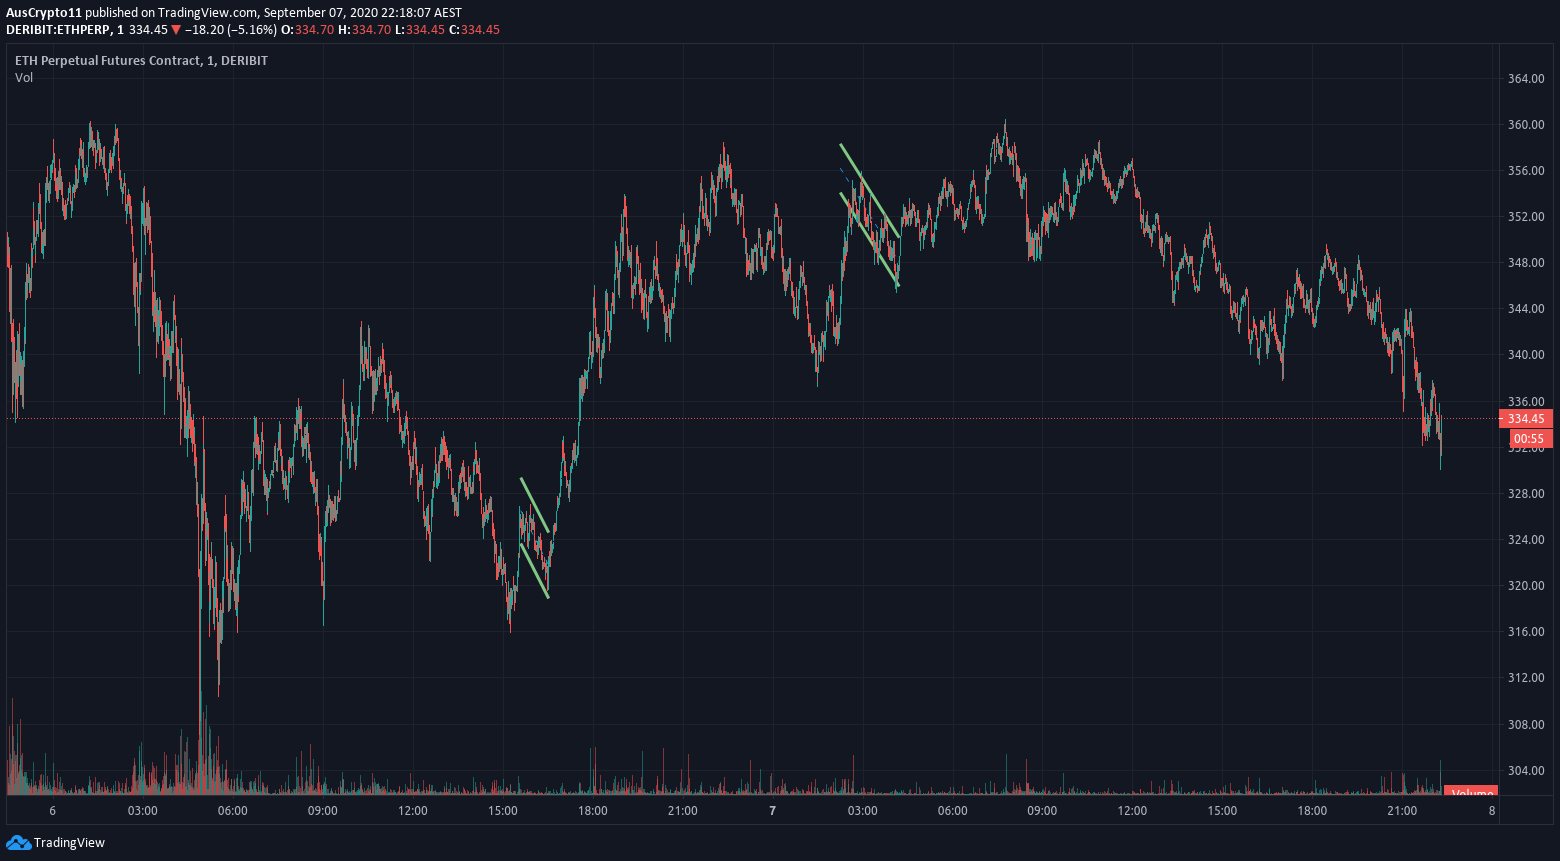
\includegraphics[width=0.8\textwidth]{fig/flag/f1.png}
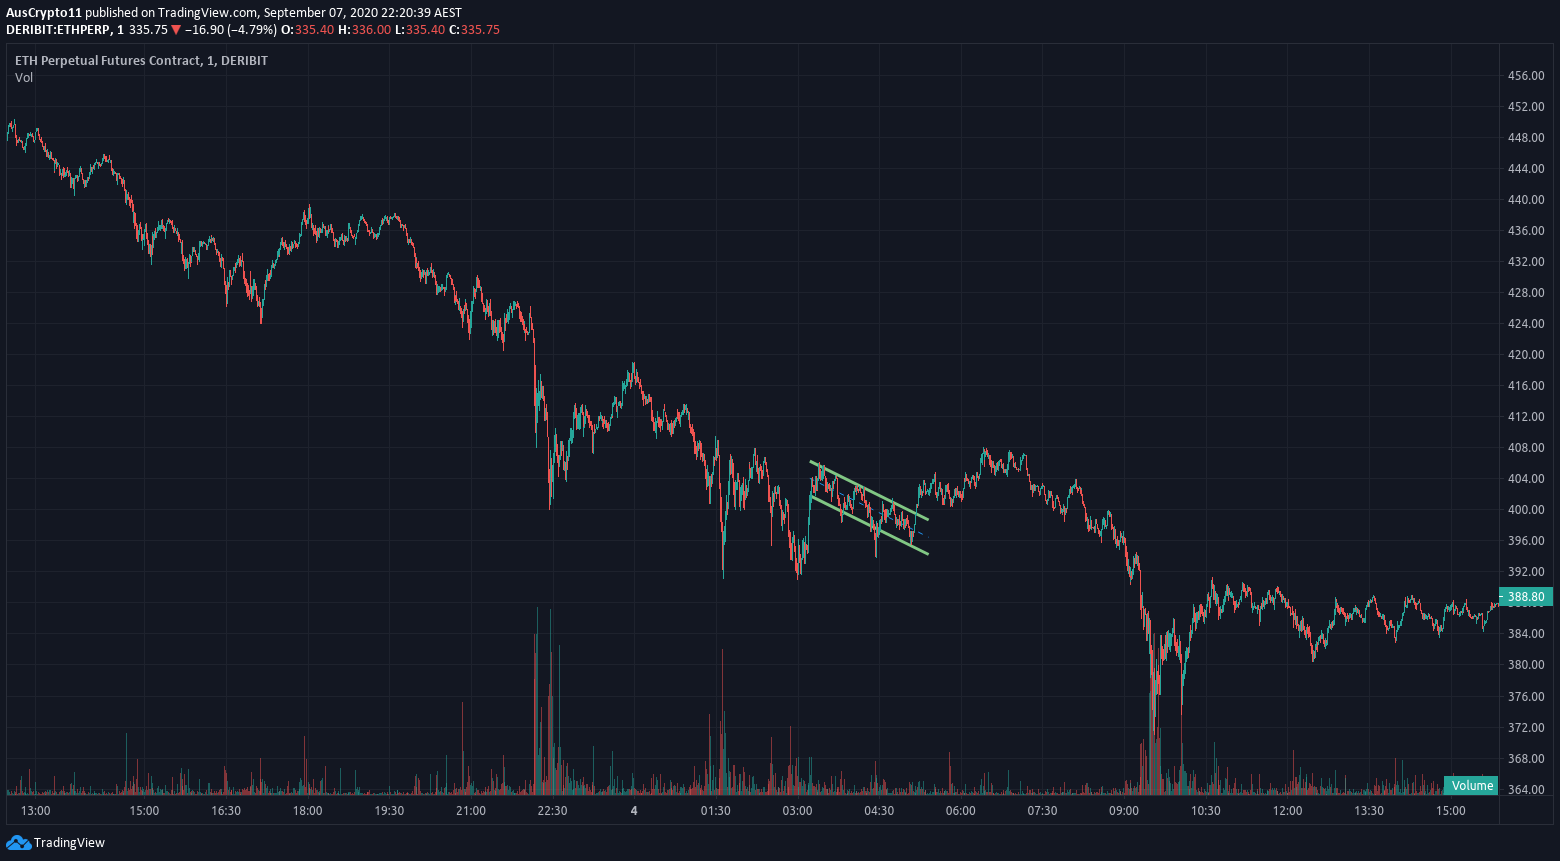
\includegraphics[width=0.8\textwidth]{fig/flag/f2.png}
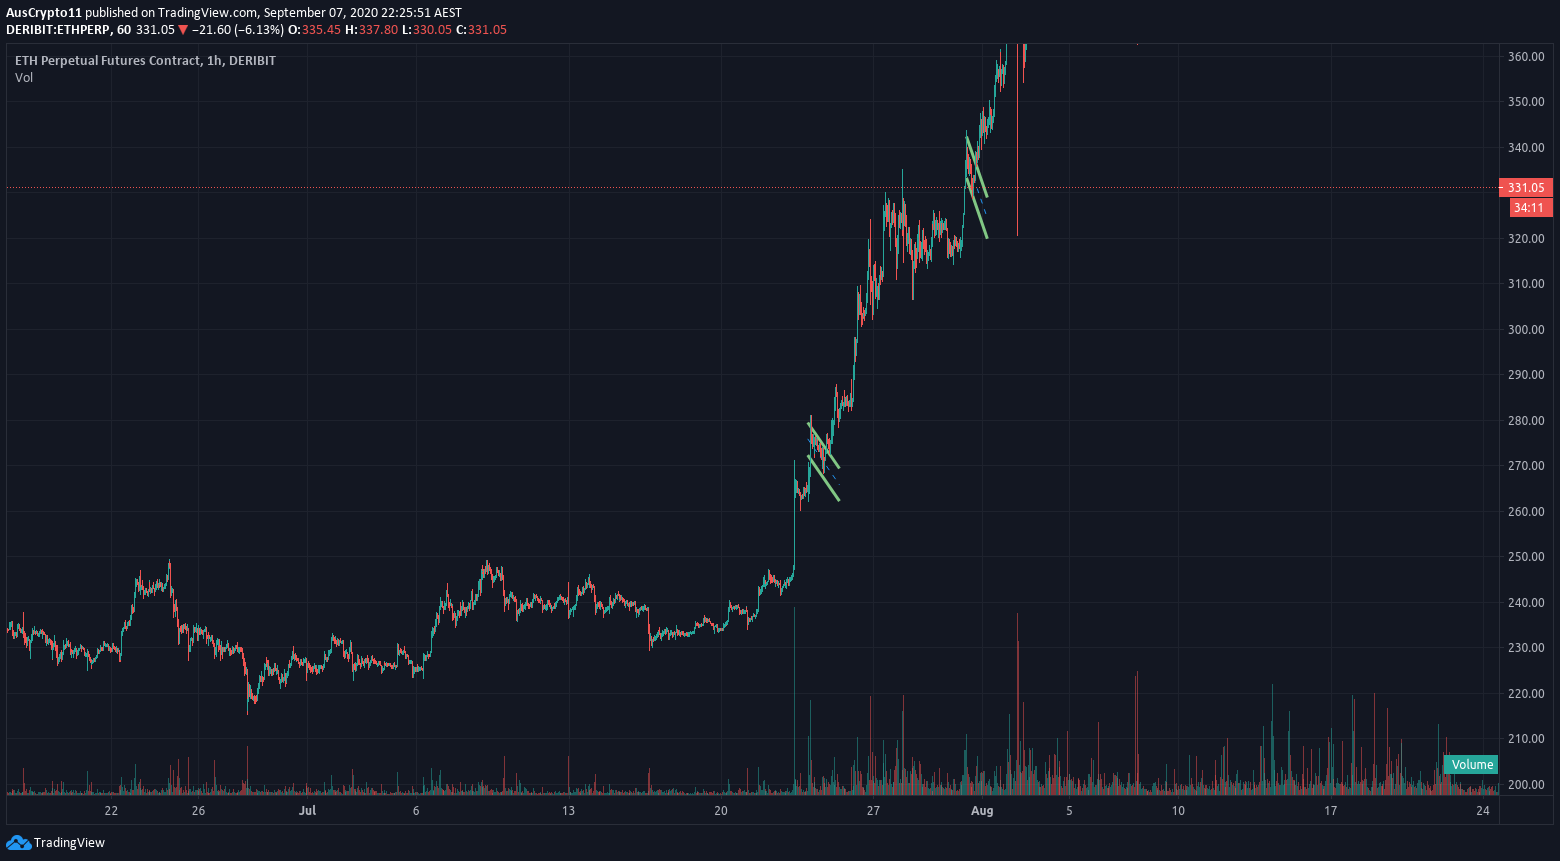
\includegraphics[width=0.8\textwidth]{fig/flag/f3.png}
\caption{Flags}
\end{figure}

\section{ Are double top / bottoms good? are head and shoulders patterns good?}
Double tops or double bottoms are not inherently good or bad. These patterns indicate if price tested a particular level. As price approaches the level there is a probability that it will reject that level or it may break through the level.

Head and shoulders patterns are also not inherently good or bad they represent A supply and demand pattern. For the Deribit perpetual futures contract there were very few head and shoulders patterns found. On the 1 min chart one could draw many head and shoulders but on this time scale these patterns can be highly subjective.
\section{ Ascending channel vs descending channels}
Ascending channels often occur immediately after a sharp move in the long direction. Descending channels are more common on larger time frames.  We can find channels on both 1 hour and 1 minute time frames. 
See examples below

\begin{figure}[H]
\center
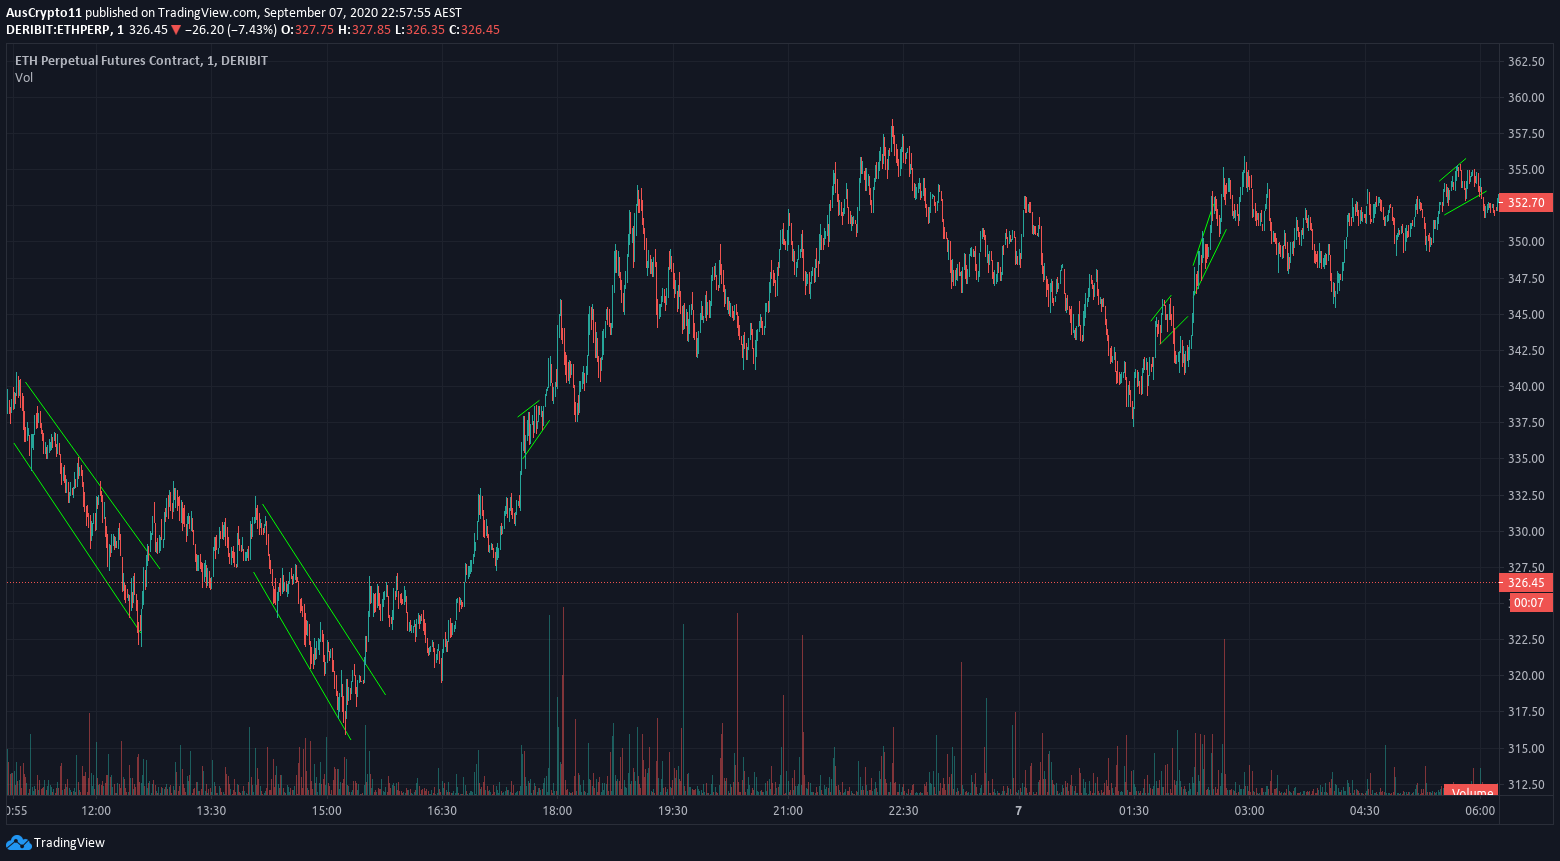
\includegraphics[width=0.8\textwidth]{fig/chan/c1.png}
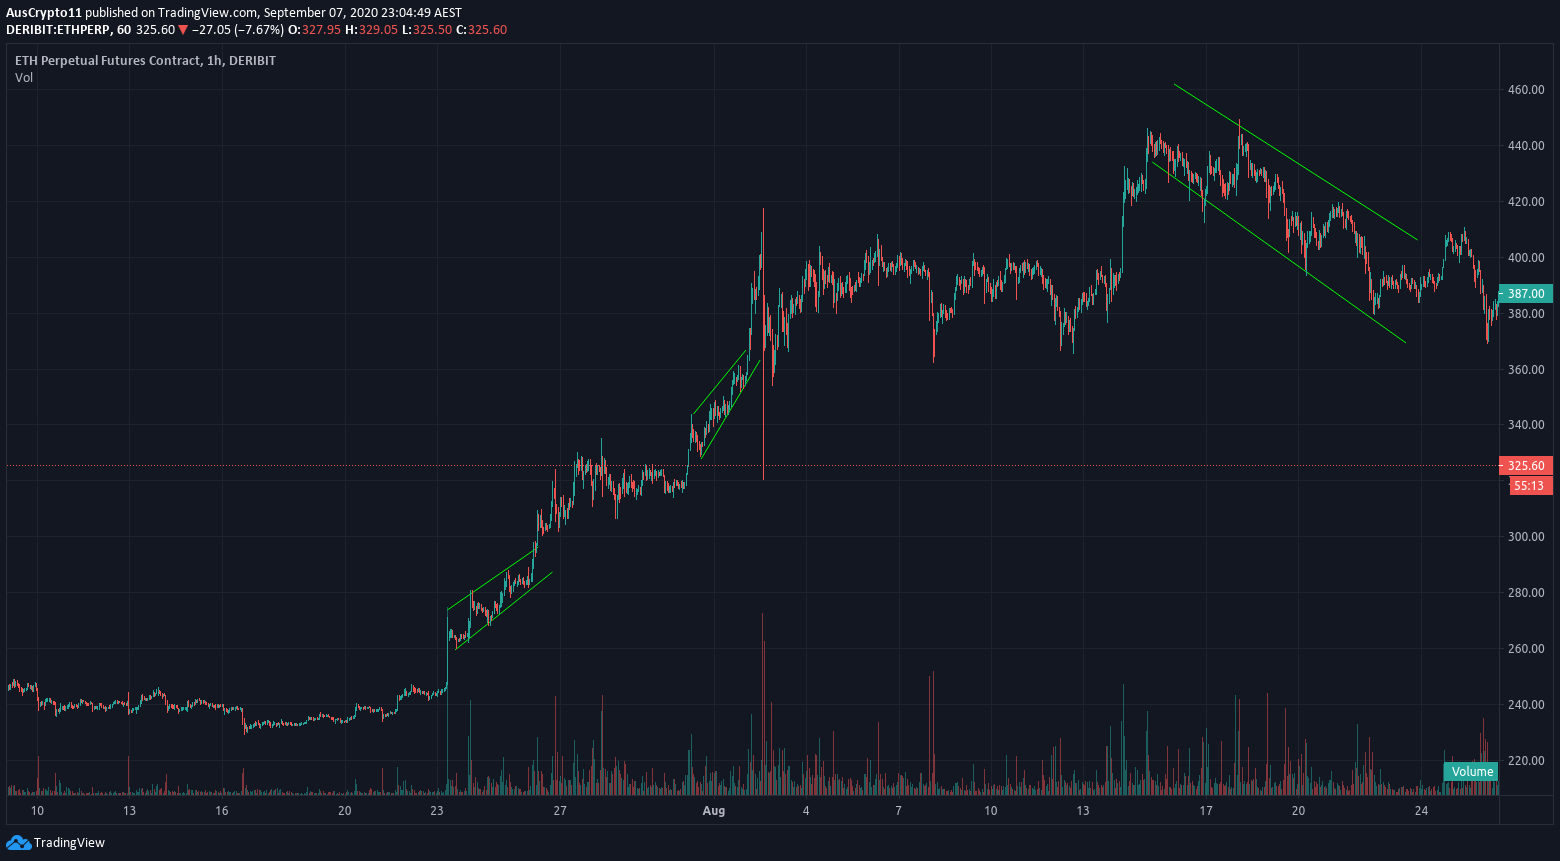
\includegraphics[width=0.8\textwidth]{fig/chan/c2.png}
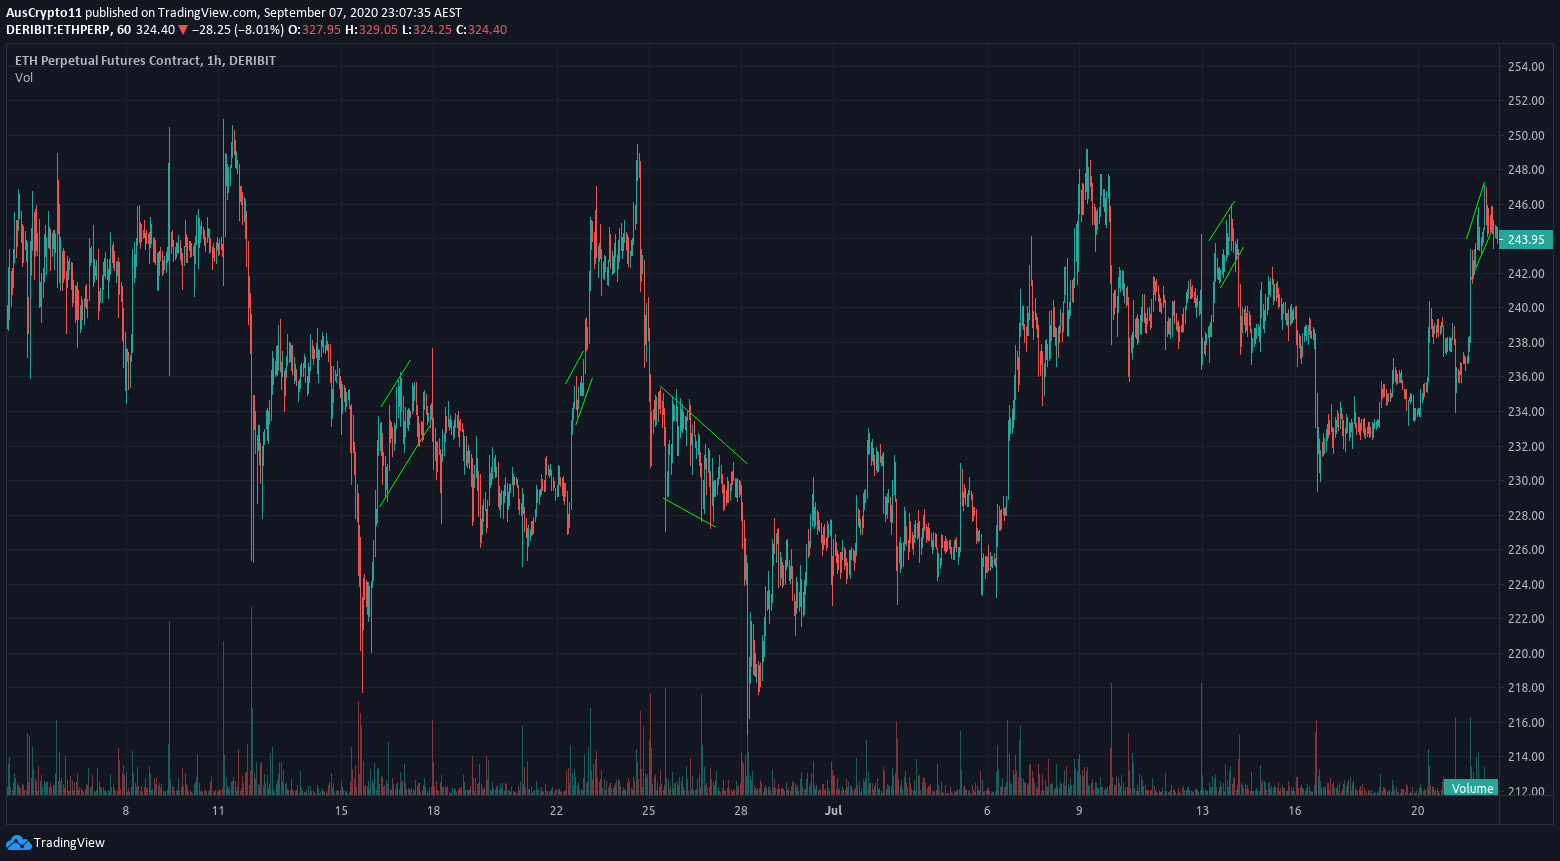
\includegraphics[width=0.8\textwidth]{fig/chan/c3.png}
\caption{Channels}
\end{figure}



\section{ Does the market fill the CME gap from the weekends trading? If so what are some statistics around this?}
Bitcoin futures contracts are traded on the Chicago Mercantile exchange (CME) The CME does not trade on weekends so there are gaps in these BTC future prices even though the crypto market is 24/7.  There are no futures contracts for ETH on the CME so we detected no gaps in the price of ETH.

At a later time we will scrape data for Bitcoin futures and provide the relevant statistics.


\section{ Are weekends more likely to trend or range?}
In order to answer this question we fit a linear regression model to each day (1011 separate linear models) . We record the absolute gradients of each day. A high absolute gradient will indicate a trend day while a low absolute gradient will indicate a range day. If the absolute gradient is exactly 1 the tread was on average 45 degrees.

Figure \ref{fig:week_trend} shows that weekend tends to trend but have less extreme moves.

\begin{figure}[H]
\center
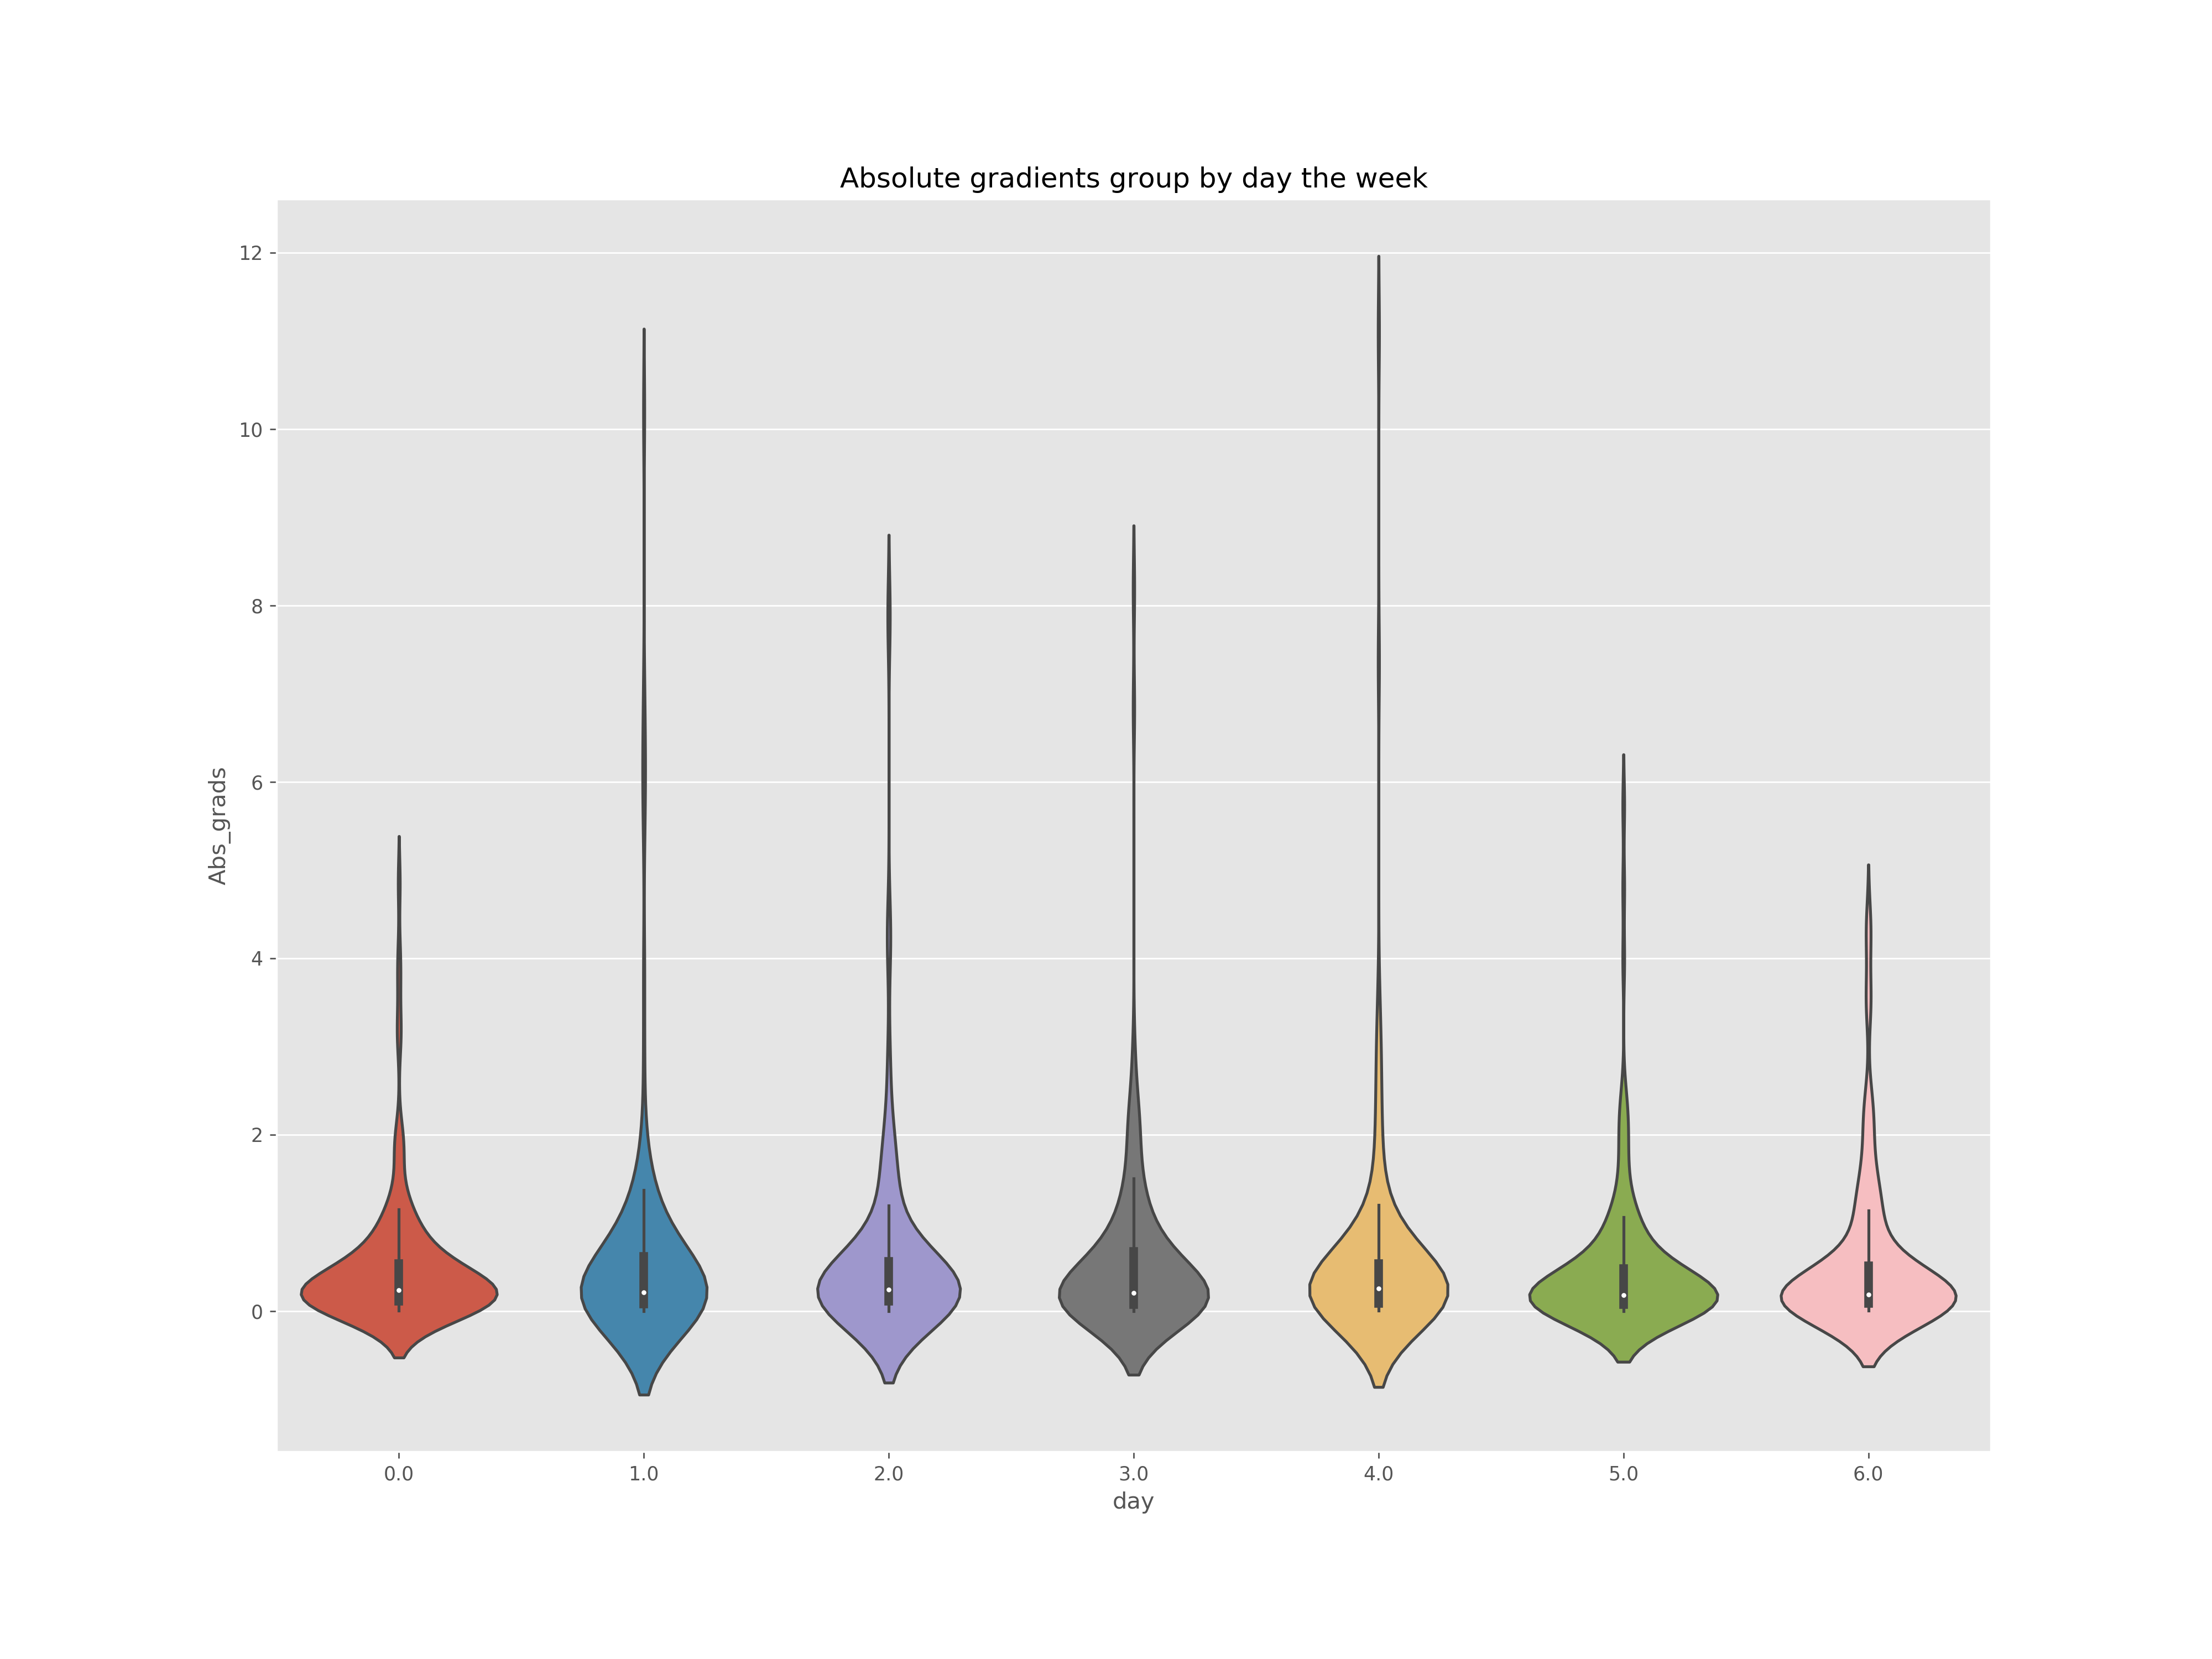
\includegraphics[width=0.9\textwidth]{fig/week_trend.png}
\caption{Volume distribution}
\label{fig:week_trend}
\end{figure}

\section{ How does changes in volume affect the market}

Qualitatively a spike in volume corresponds to a big move up or a big move down.
Qualitatively a spike in volume corresponds to a big move up or a big move down. Lower volume levels correspond to a ranging market.

This is confirmed below with correlation matrix. We see that the correlation between volume and absolute returns is 0.412379. \\
\begin{tabular}{lrrrrr}
\toprule
{} &     close &   returns &   abs\_ret &    std\_24 &    volume \\
\midrule
close   &  1.000000 &  0.012390 &  0.528951 &  0.720088 &  0.059851 \\
returns &  0.012390 &  1.000000 & -0.021348 & -0.003667 & -0.006424 \\
abs\_ret &  0.528951 & -0.021348 &  1.000000 &  0.662447 &  0.412379 \\
std\_24  &  0.720088 & -0.003667 &  0.662447 &  1.000000 &  0.318054 \\
volume  &  0.059851 & -0.006424 &  0.412379 &  0.318054 &  1.000000 \\
\bottomrule
\end{tabular}
\section{ Does volatility drop and volume drop at the same time or do they move inline}
From the table there is a strong correlations (0.318054) between std (volatility) and volume. In short volatility and volume move together.

Figure \ref{fig:rvs} shows the relationship between volatility, volume and return.
\begin{figure}[H]
\center
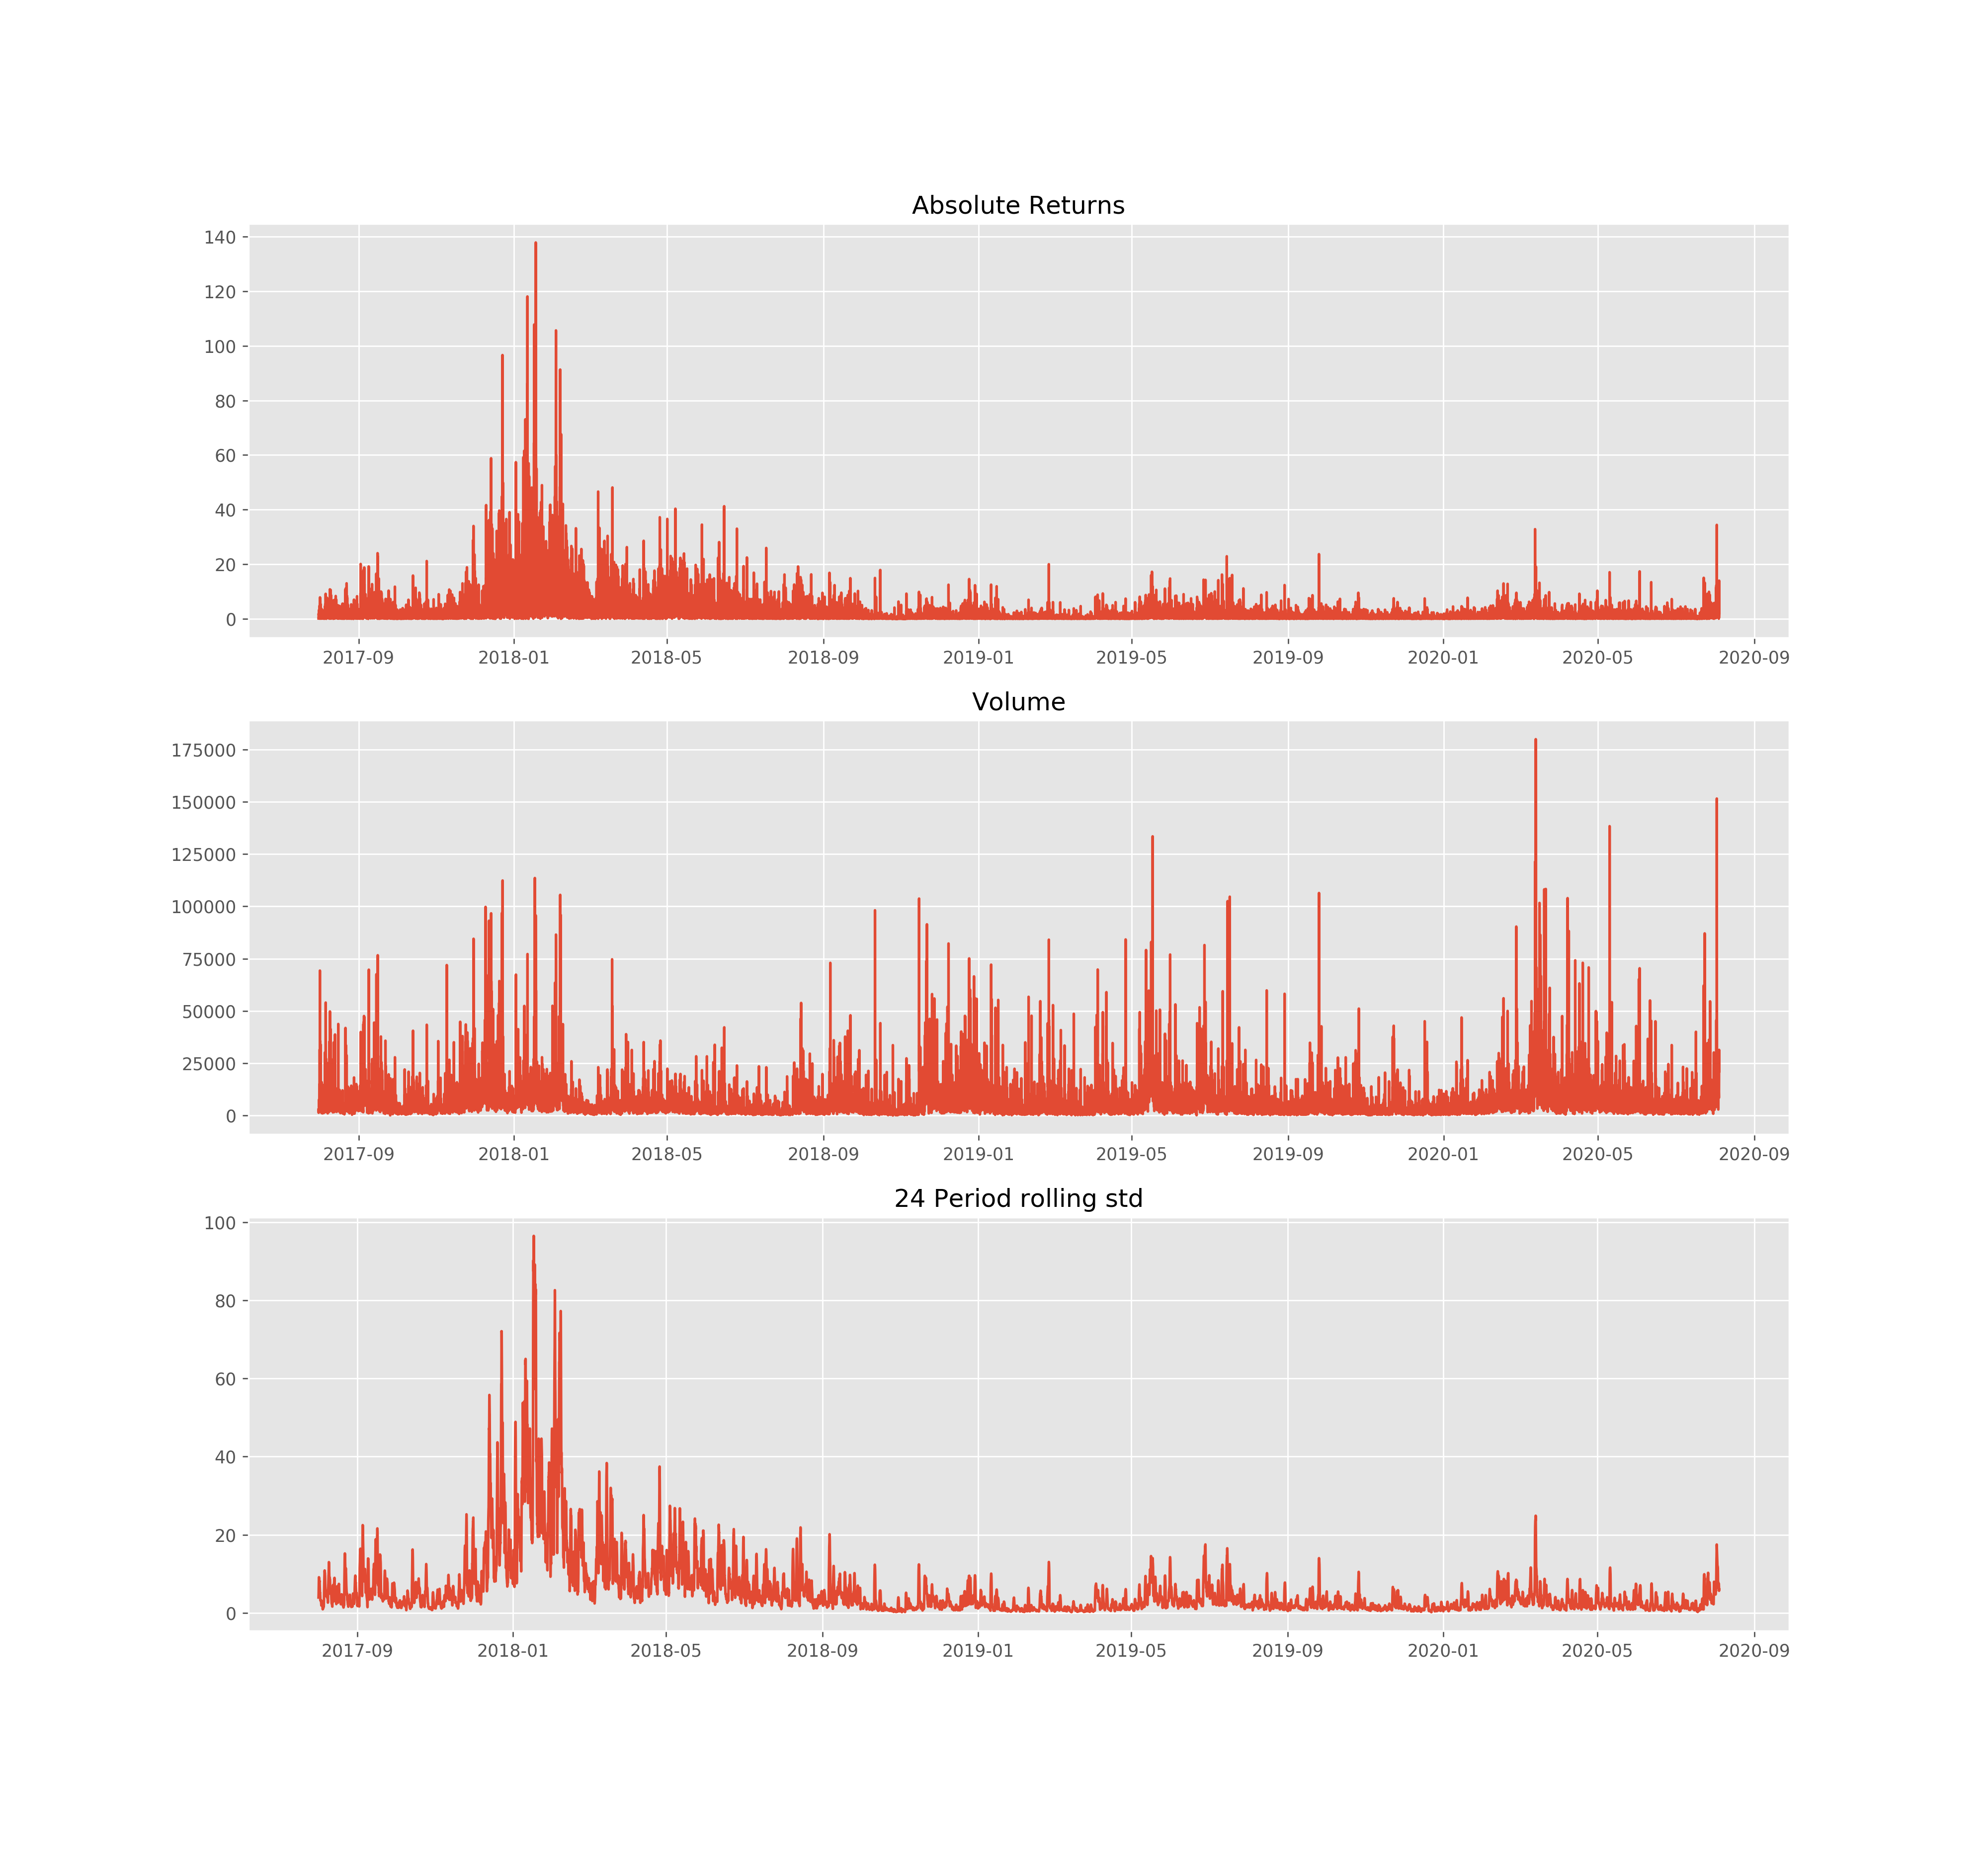
\includegraphics[width=0.9\textwidth]{fig/rvs.png}
\caption{Absolute Returns, volume and volatility }
\label{fig:rvs}
\end{figure}
\section{ Do liquidations occur with or against the trend}

Figure \ref{fig:liq} shows long and short liquidations compared with open interest and price. The data is taken from coinalyze. We have 60 minute candles for the past month. 

We see that liquidations occur against the train for example if long positions are liquidated this is followed by price drop.
\begin{figure}[H]
\center
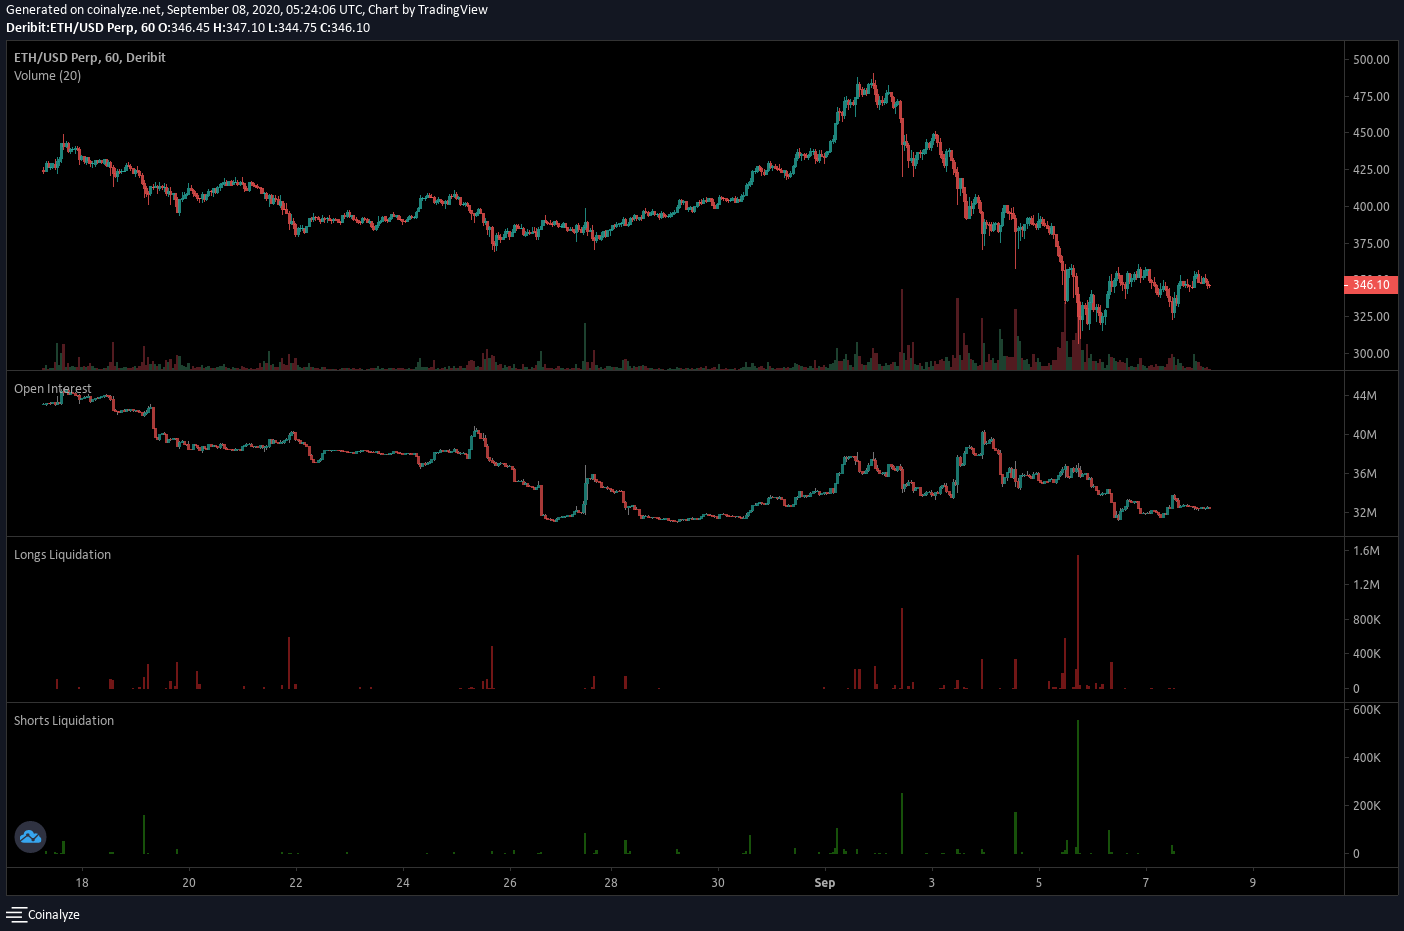
\includegraphics[width=0.9\textwidth]{fig/liq.png}
\caption{Long and short liquidations compared with open interest and price }
\label{fig:liq}
\end{figure}
\section{ When it ranges how big are the moves and what size reversions do they have?}
\begin{itemize}
\item We define a ranging market to be one where the volume is below 50000.
\item Given this volume threshold we group the data in range sections separated by trend sections. 
\end{itemize}
Figure \ref{fig:ras} show illustrates a few range sections. 
\begin{figure}[H]
\center
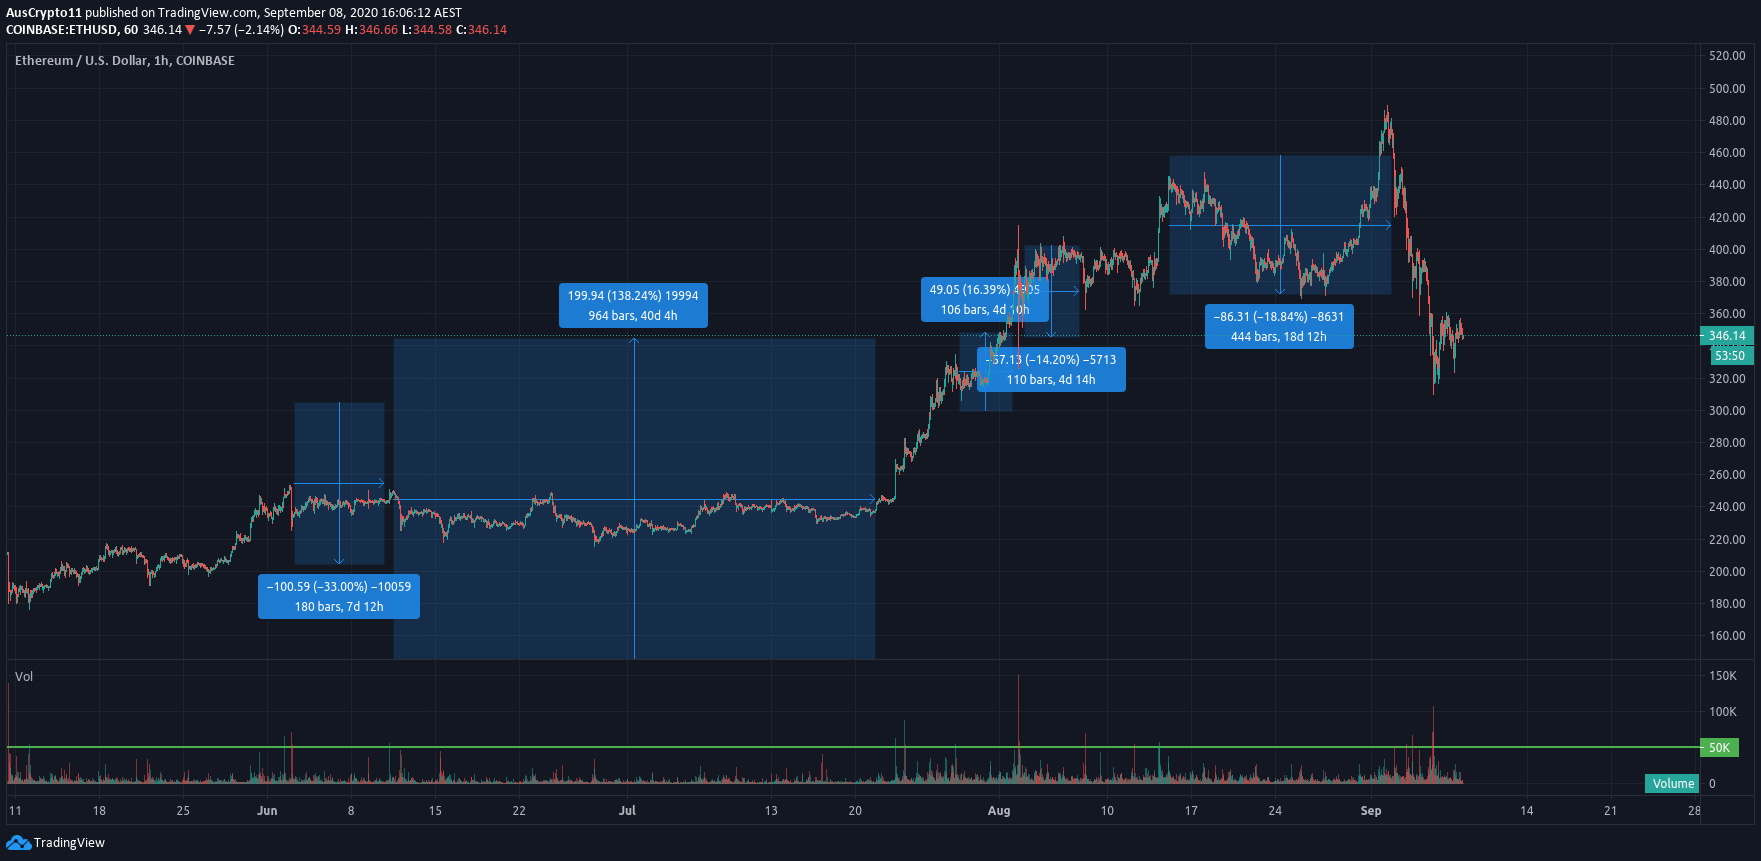
\includegraphics[width=0.9\textwidth]{fig/ras.png}
\caption{A few range sections}
\label{fig:ras}
\end{figure}

Here is the algorithm that separates trend and range days.

\begin{verbatim}
trend_days = np.argwhere(df["is_range"].values==False).flatten()
start = 0
end = 0
range_section = []
for elem in trend_days:
    end = elem
    if np.abs(start - end) == 0 :
        start = end + 1
        continue
    else:
        range_section.append(df.iloc[start:end])
        start = end + 1
\end{verbatim}
For each range section we find the volatility. This will us use a way to measure the average reversion size.

\begin{verbatim}
The average std for all range sections 16.126381667472764
\end{verbatim}


\section{ When it goes quiet what sort of ranges and volumes does it do right before a big move?}
This question follows on from the last question. We see in Figure \ref{fig:rvs} that absolute returns volume and volatility are all correlated. Thus, before a big move we see low volatility and low volume. 

Here are the mean ranges and volume for the range sections define in the previous question.
\begin{verbatim}
range        4.548437
volume    5695.183314
\end{verbatim}
\section{ When we have days of abnormally low volume what type of days do we see after this?}
Below is a list of days with the lowest volume.
\begin{verbatim}
2018-11-11     725.863348
2018-07-29     763.086708
2018-10-28     893.016279
2019-12-08     971.434971
2018-07-22    1033.791602
2019-03-24    1046.961928
2019-12-22    1099.794516
2019-11-03    1140.718775
2018-11-12    1146.788031
2019-11-10    1151.447176
\end{verbatim}
\begin{itemize}
\item 2018-11-11 : It ranged for the next week then had a massive dump.
\item 2018-07-29 : It ranged for half a week then dumped.
\item 2018-10-28 : It ranged for the next 2 weeks then had a massive dump.
\item 2018-07-22 : It ranged for the next 2 weeks then dumped.
\item 2019-03-24 : It ranged for the next 2 weeks then had a massive pump.
\item 2019-12-22 : It ranged for the next 3 weeks then had a small pump.
\end{itemize}

In summary when we have days of abnormally low volume price will range for about 1.5 weeks then pump or dump.

\section{ Once it has a big move (define this) what does the following 5 days look like}
Big move will measured by the re sampled daily range.
The list below shows the biggest moves.
\begin{verbatim}
date_time     range
2018-01-17    80.199583
2018-01-18    63.816667
2018-01-11    54.014583
2018-02-06    50.523333
2018-01-16    47.949167
2018-02-02    43.935833
2018-01-10    43.792917
2018-01-09    41.279167
2017-12-23    40.481667
\end{verbatim}
\begin{itemize}
\item 2018-01-17 : consolidation followed
\item 2018-01-11 consolidation followed for 5 days then dumped
\item 2017-12-23 : This was a big wick down. After this candle price ranged.
\end{itemize}
We now look at big move in 2020
\begin{verbatim}
date_time     range
2020-03-13    13.134583
2020-08-02    12.952917
2020-08-04     8.125833
2020-03-12     7.845417
2020-08-03     7.157083
2020-02-17     6.997917
2020-02-27     6.396250
2020-02-13     6.267500
2020-03-09     6.168333
2020-07-28     6.036250
2020-03-14     6.000417
\end{verbatim}
\begin{itemize}
\item 2020-03-13 : ranging followed
\item 2020-08-02 : This was a big wick candle ranging followed
\item 2020-08-04 : ranging followed.
\end{itemize}

\section{ What does the next 12, 24 hours look like after a large move?}

This question follows on from the last question. Looking at the big moves defined in the previous question, we see that price ranges  during the next 12 to 24 hours. 


\section{ Are moves more likely to retrace or continue on longs or shorts?}

We look at data from August to present day. Qualitatively after a long or short move the market is more likely to retrace. This is because the market is mostly ranging. The price will continue in its long or short position if it is part of a bigger macro trend. 

Figure \ref{fig:ret2} shows several instances of retracements
\begin{figure}[H]
\center
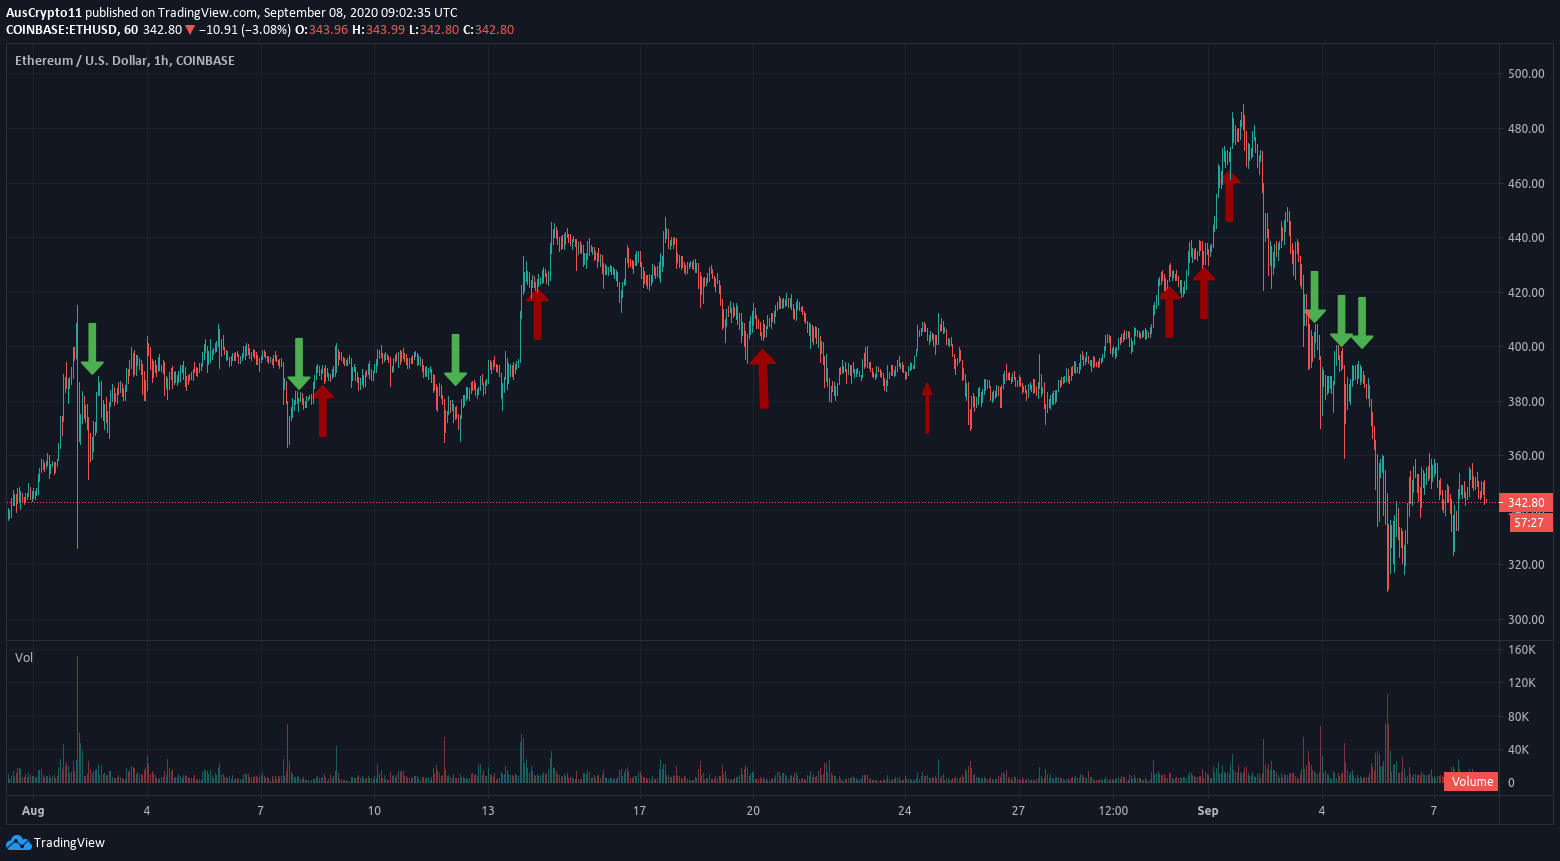
\includegraphics[width=0.9\textwidth]{fig/ret2.png}
\caption{Retracements}
\label{fig:ret2}
\end{figure}


\section{ Look into what vwap is, put it on your chart and see does vwap work? is it more active in ranging or trending, more volatile or less volatile.}
VWAP  stands for volume weighted average price. For a specified time period (on trading view it is one day) 

$$vwap = \frac{\sum (price * volume)}{\sum volume}$$

It is similar to a weighted moving average but the weights are given by the volume.

Logically, spikes in volume will affect the vwap more. This does not necessarily imply high volatility or a strong trend will affect the vwap. The formula above states that it is only dependent on price and volume.

The Vwap can tell the trader if he entered or exited at a good price.  Ideally, one should buy below the Vwap and sell above the vwap.

Figure \ref{fig:vwap} shows VWAP on the 1 min chart
\begin{figure}[H]
\center
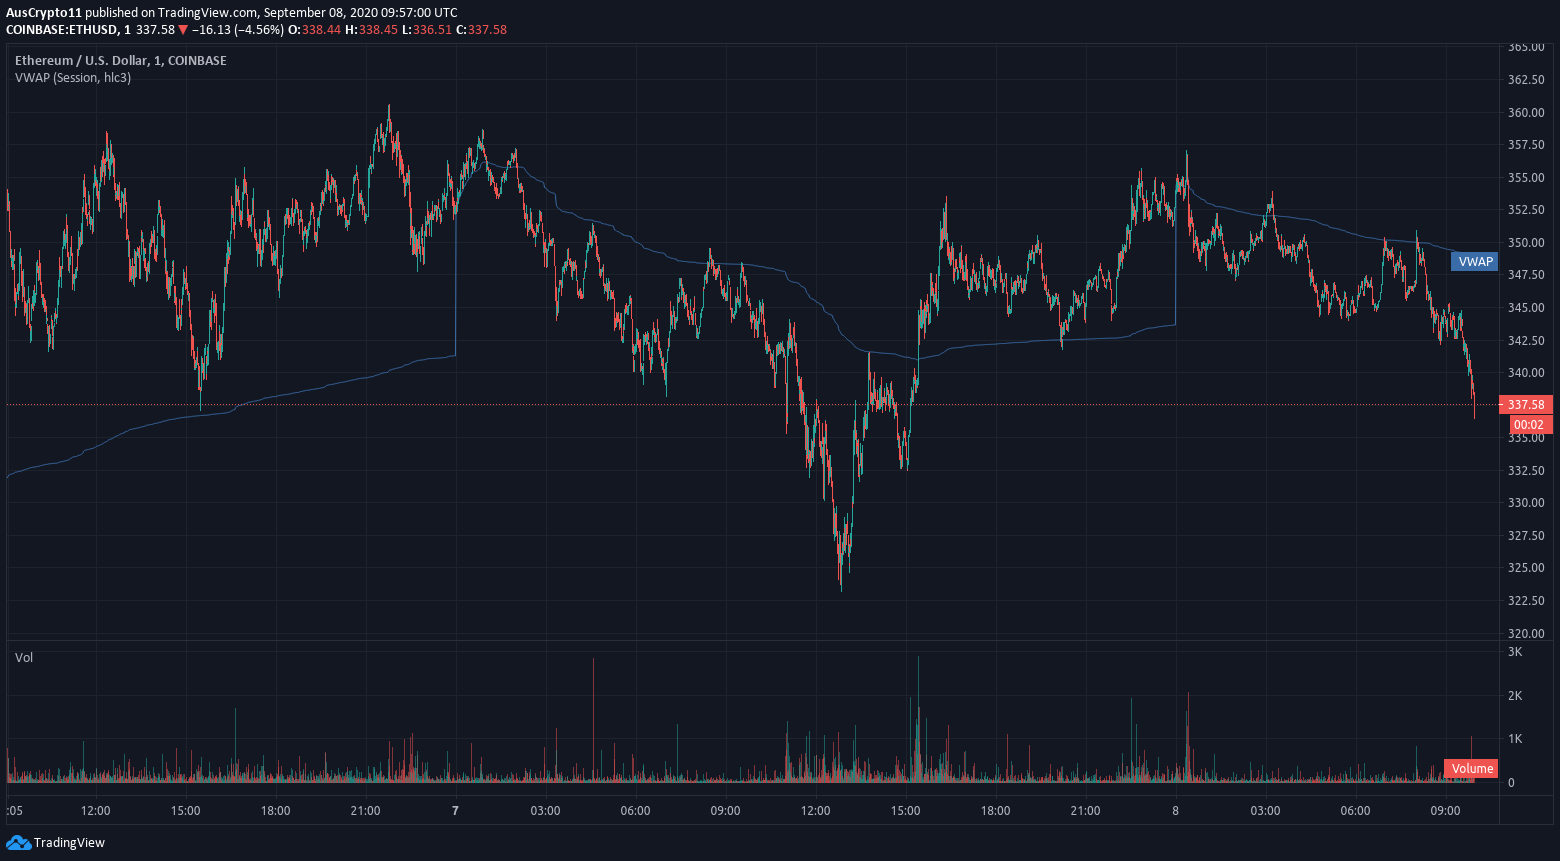
\includegraphics[width=0.9\textwidth]{fig/vwap.png}
\caption{Retracements}
\label{fig:vwap}
\end{figure}

\section{ Are the euro sessions more prone to reverse or continue the move?}
To answer this question we will investigate stationarity of closing prices in the Euro and us session.

To find the gradient of each we use the following algorithm

\begin{verbatim}
m_euro = np.zeros(len(list_by_date_euro))
for i in range(len(list_by_date_euro)):
    X = np.array(range(len(list_by_date_euro[i]["close"])))
    X_bar = X.mean()
    X_bar
    Y = list_by_date_euro[i]["close"].values
    Y_bar = Y.mean()
    m_euro[i] = np.sum((X - X_bar)* (Y - Y_bar))/np.sum((X - X_bar)**2)
\end{verbatim}

Figure \ref{fig:grad_euro} show the distribution of gradients for the Euro session 

\begin{figure}[H]
\center
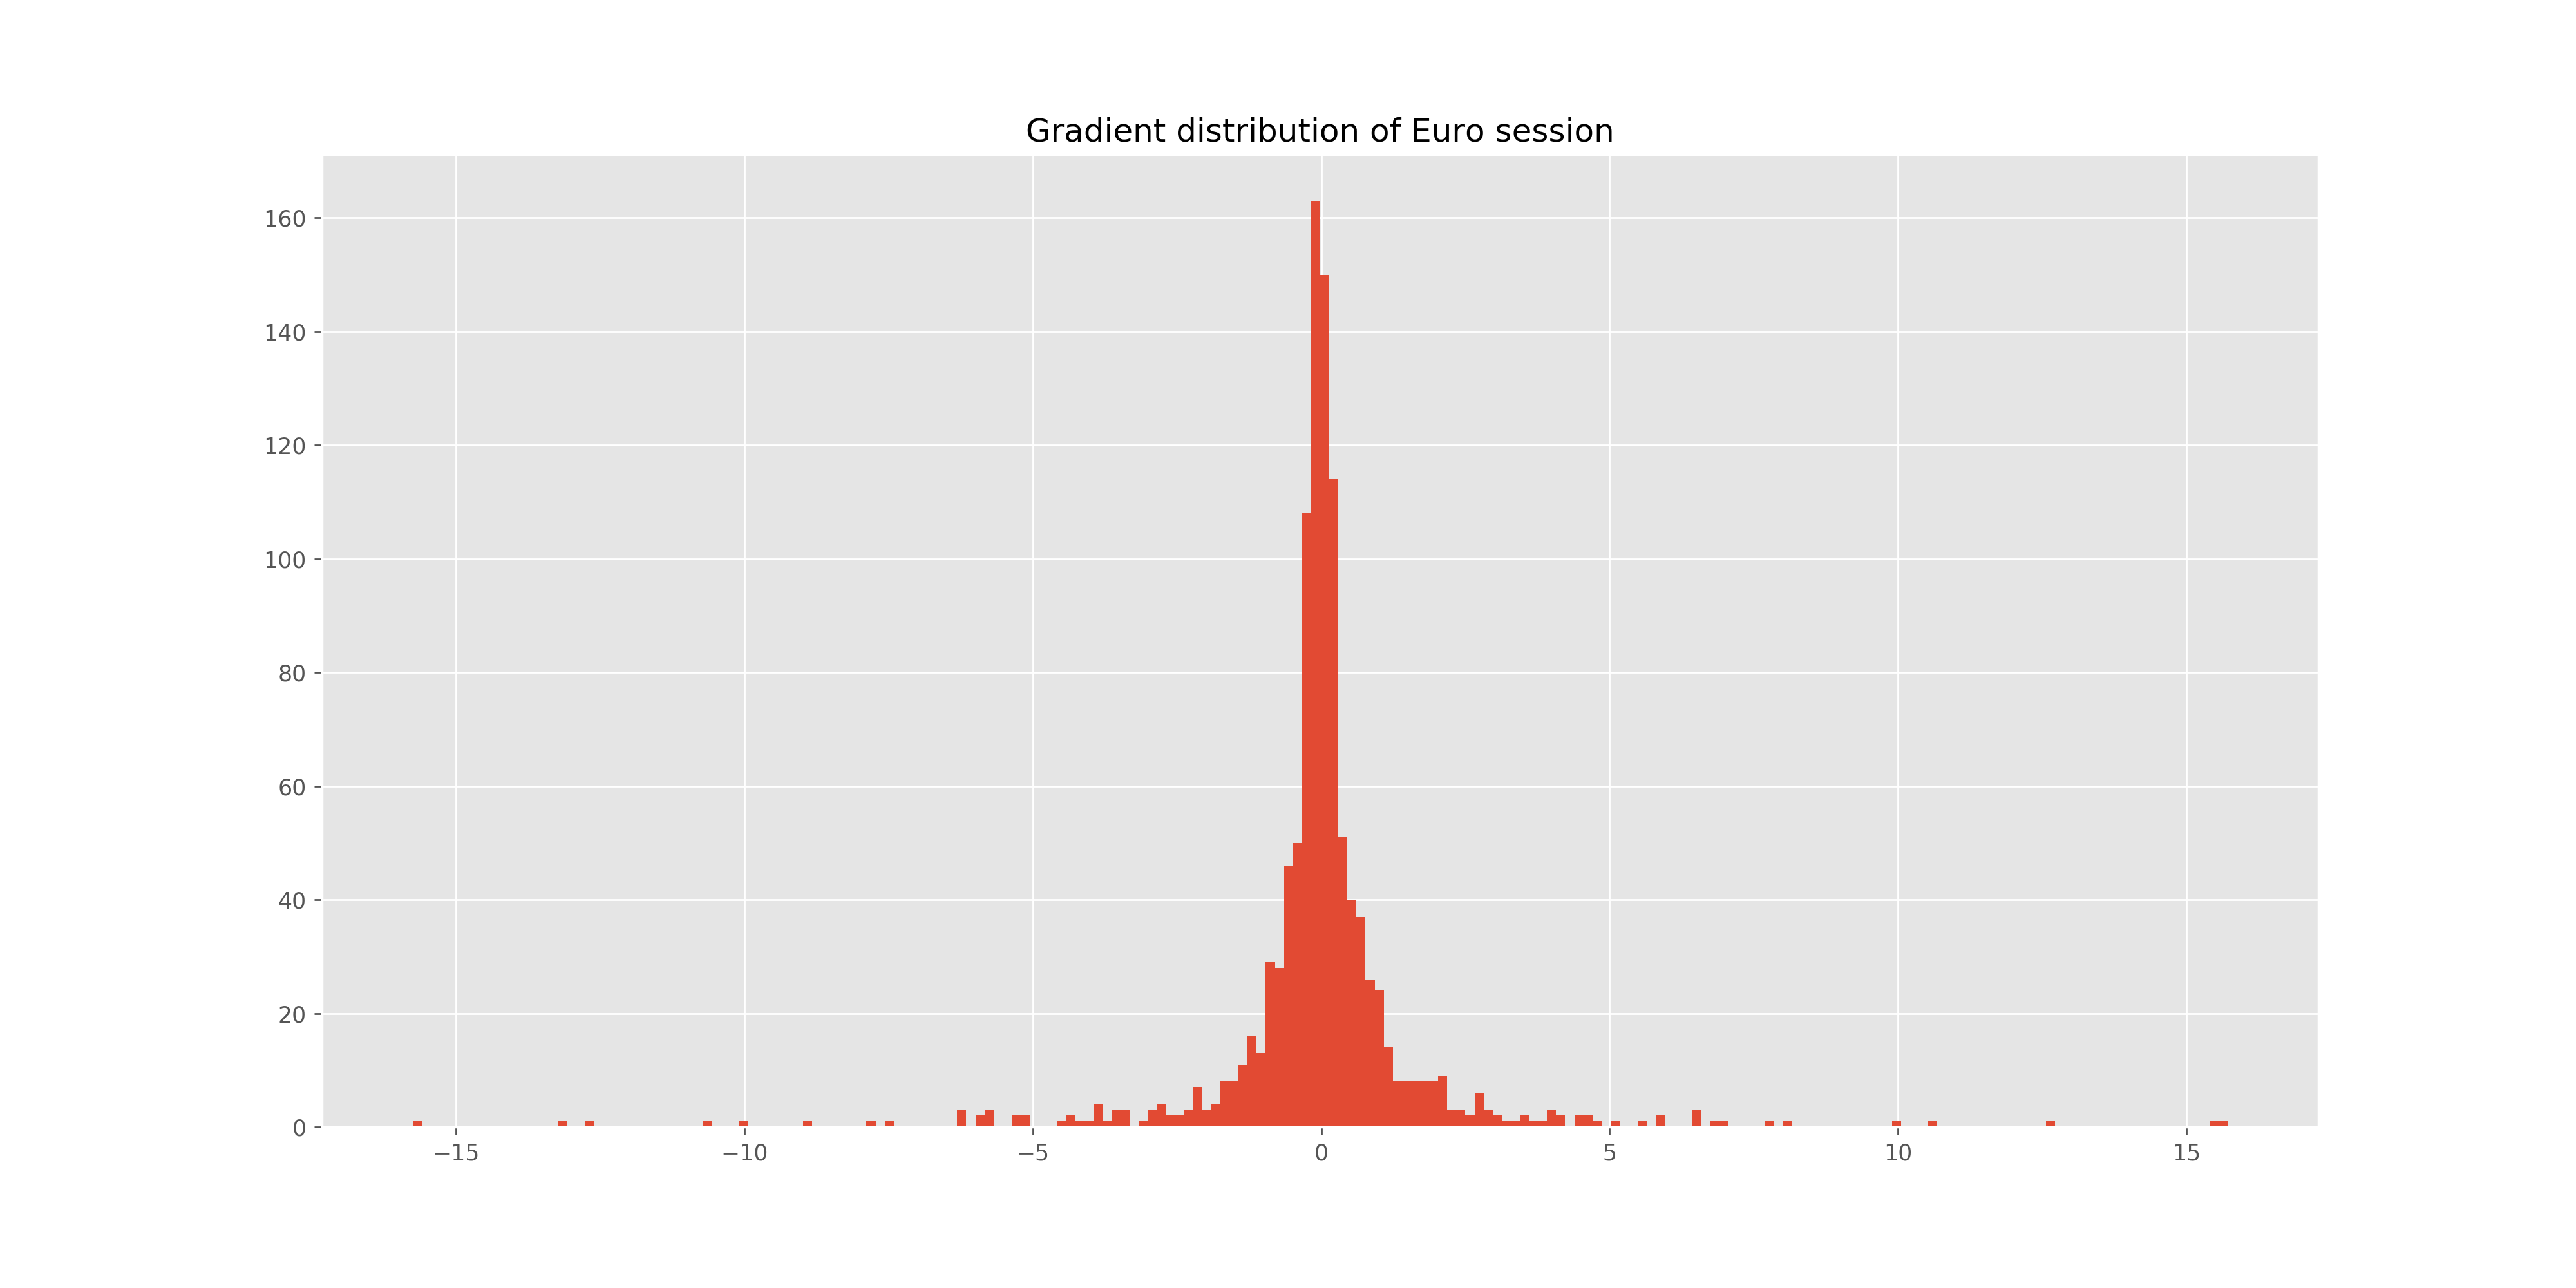
\includegraphics[width=0.9\textwidth]{fig/grad_euro.png}
\caption{Gradient distribution for the Euro session}
\label{fig:grad_euro}
\end{figure}
The further away gradients are from 0 the more likely price trended.
\section{ Are the usa sessions more prone to reverse or continue the move?}
We perform the same analysis for the usa session.

From Figure \ref{fig:grad_usa} we can conclude that there are more extreme down with trends during the US session.
\begin{figure}[H]
\center
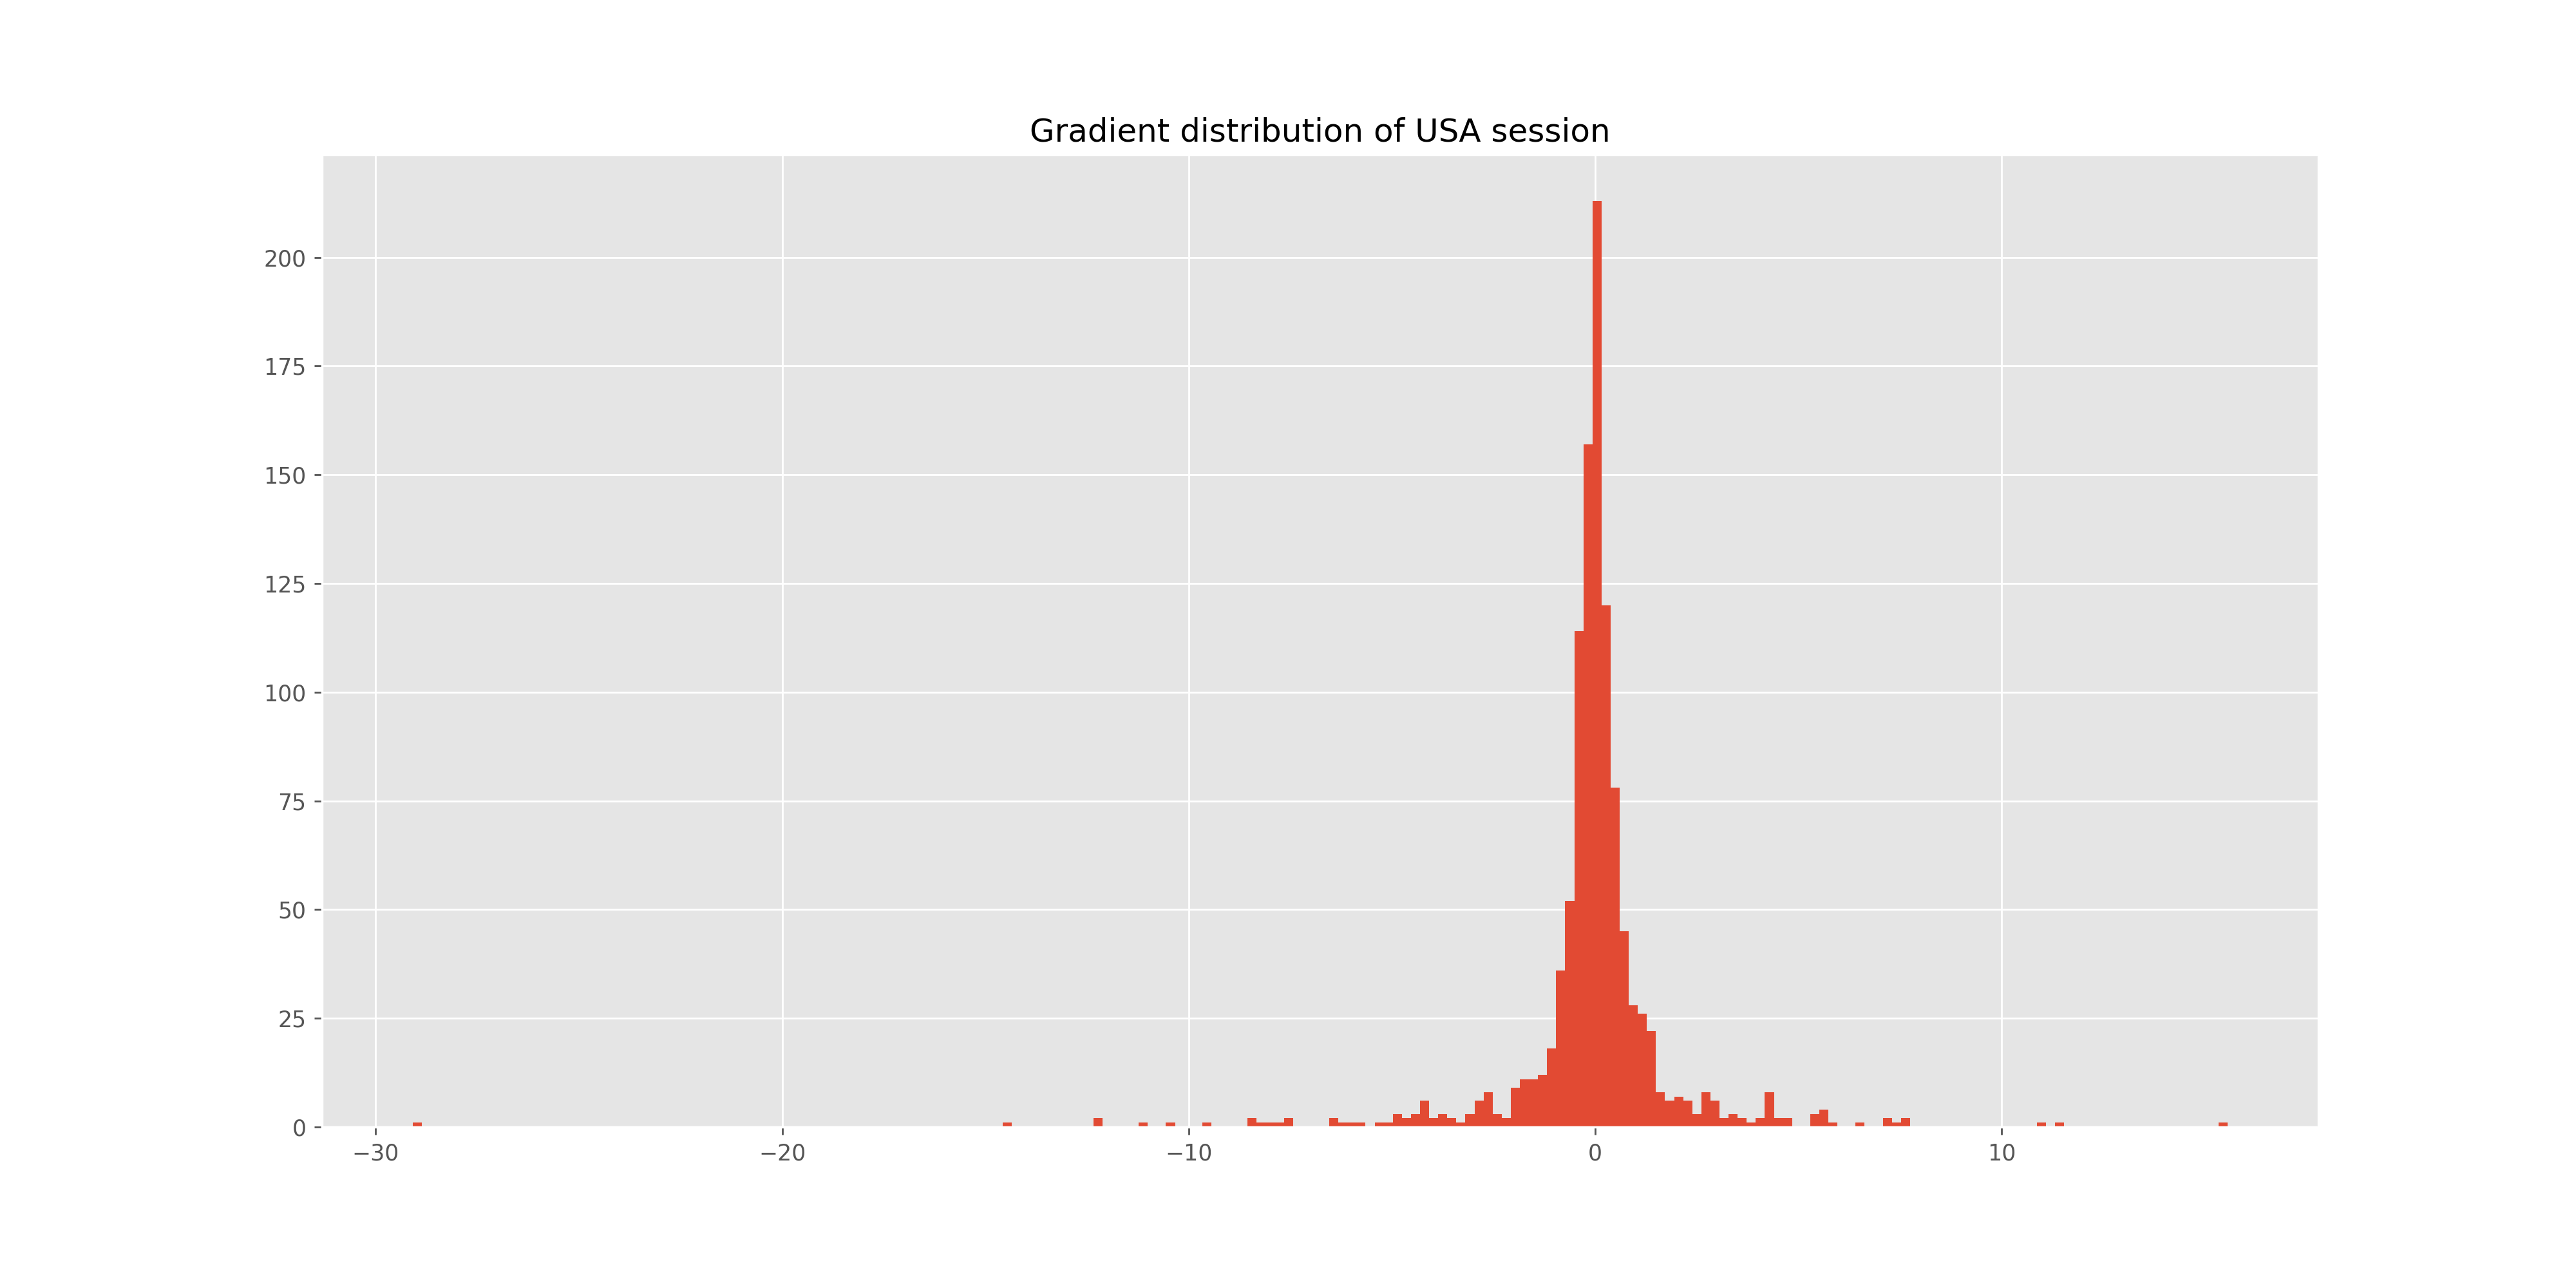
\includegraphics[width=0.9\textwidth]{fig/grad_usa.png}
\caption{Gradient distribution for the USA session}
\label{fig:grad_usa}
\end{figure}

\section{ How responsive is the market to current SFL levels? (tradingview)}
SFL levels include Daily weekly monthly or yearly open and closed. From observation I found that SFL levels work best with line charts. 

Price seems to respect the weekly open and close. Daily SFL levels are often crossed.

Figure \ref{fig:sfl} shows the SFL levels for the past 3 months.

\begin{figure}[H]
\center
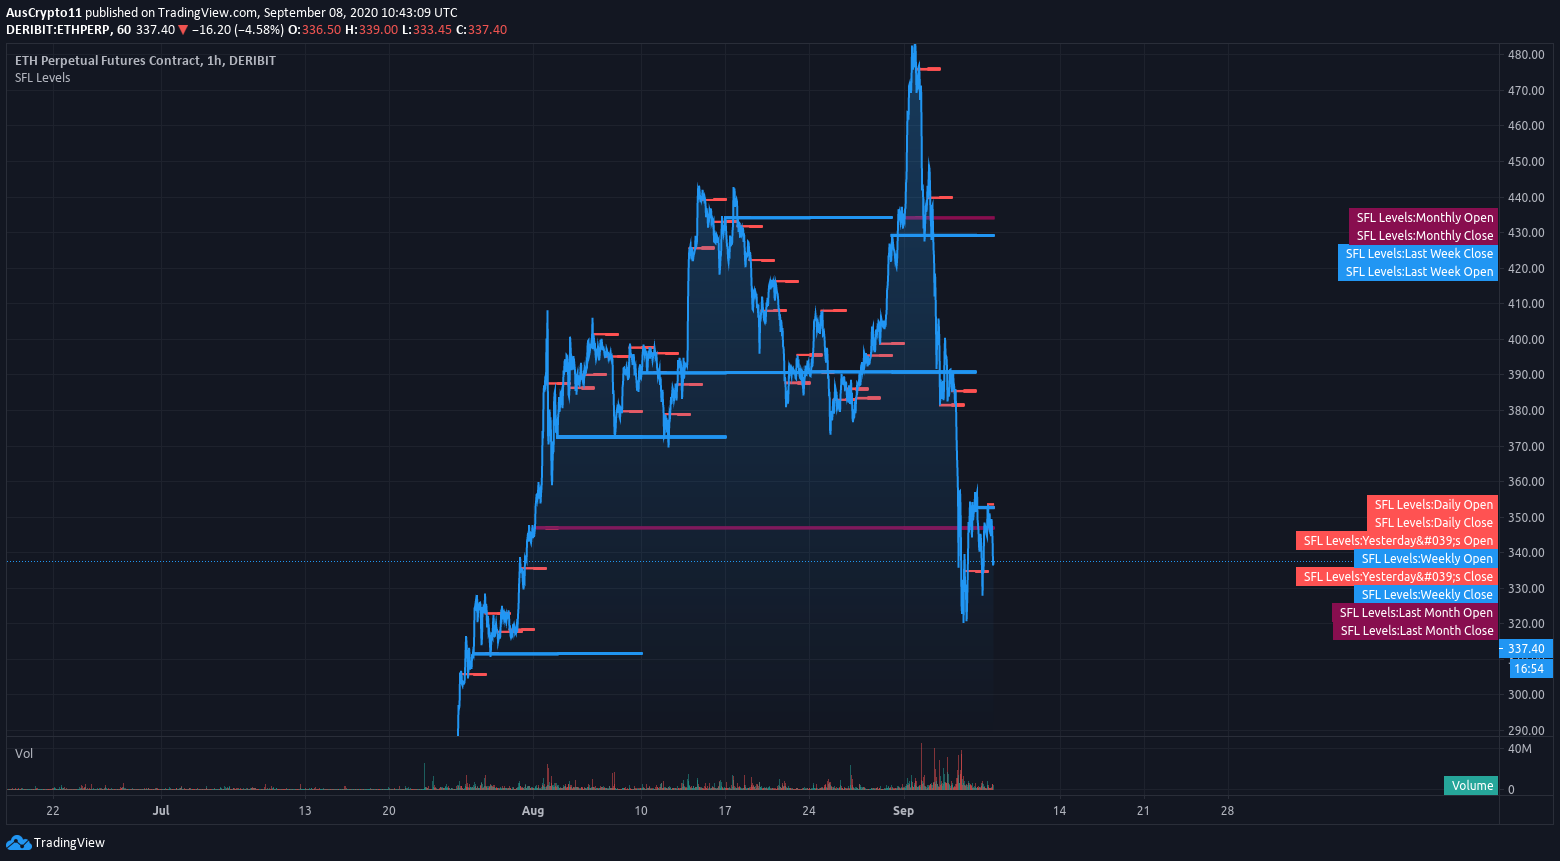
\includegraphics[width=0.9\textwidth]{fig/sfl.png}
\caption{SFL levels}
\label{fig:sfl}
\end{figure}

\section{ Which SFL levels are the most important? }
\begin{itemize}

\item For the 1 hour time frame the weekly acid levels are the most important.
\item For the daily time frame the monthly SFL levels are most relevant.

\end{itemize}

\section{ Does price respect past SFL levels?}
Price does respect past SFL levels.  This is most predominantly seen for the weekly SFL levels on the one hour chart. 